\documentclass[12pt,letterpaper]{article}
\usepackage[top=0.85in,left=1in,footskip=0.75in,marginparwidth=2in]{geometry}

% use Unicode characters - try changing the option if you run into troubles with special characters (e.g. umlauts)
\usepackage[utf8]{inputenc}

% clean citations
\usepackage{cite}

% hyperref makes references clicky. use \url{www.example.com} or \href{www.example.com}{description} to add a clicky url
\usepackage{nameref,hyperref}

% line numbers
\usepackage[right]{lineno}

% improves typesetting in LaTeX
\usepackage{microtype}
\DisableLigatures[f]{encoding = *, family = * }

% text layout - change as needed
\raggedright
\setlength{\parindent}{0.5cm}
\textwidth 6.5in 
\textheight 9in
\renewcommand{\baselinestretch}{1.5}

% use adjustwidth environment to exceed text width (see examples in text)
\usepackage{changepage}

% adjust caption style
\usepackage[aboveskip=1pt,labelfont=bf,labelsep=period,singlelinecheck=off]{caption}

% remove brackets from references
\makeatletter
\renewcommand{\@biblabel}[1]{\quad#1.}
\makeatother

% headrule, footrule and page numbers
\usepackage{lastpage,fancyhdr,graphicx}
\usepackage{epstopdf}
\pagestyle{myheadings}
\pagestyle{fancy}
\fancyhf{}
\rfoot{\thepage/\pageref{LastPage}}
\renewcommand{\footrule}{\hrule height 2pt \vspace{2mm}}
\fancyheadoffset[L]{2.25in}
\fancyfootoffset[L]{2.25in}

% use \textcolor{color}{text} for colored text (e.g. highlight to-do areas)
\usepackage{color}

% define custom colors (this one is for figure captions)
\definecolor{Gray}{gray}{.25}

% this is required to include graphics
\usepackage{graphicx}
\graphicspath{{../figures/}}

% use if you want to put caption to the side of the figure - see example in text
\usepackage{sidecap}

% use for have text wrap around figures
\usepackage{wrapfig}
\usepackage[pscoord]{eso-pic}
\usepackage[fulladjust]{marginnote}
\reversemarginpar

% document begins here
\begin{document}
\vspace*{0.35in}

% title goes here:
\begin{flushleft}
{\Large
\textbf\newline{Are essential genes conserved?}
}
\newline
% authors go here:
\\
%Fatemeh Ashari Ghomi\textsuperscript{1},
%Paul P. Gardner\textsuperscript{1,*},
%Lars Barquist\textsuperscript{2}
%\\
%\bigskip
%\bf{1} University of Canterbury
%\\
%\bf{2} Wurzburg University
%\\
%\bigskip
%* paul.gardner@canterbury.ac.nz

\end{flushleft}

\section*{Abstract}
%Fitting multiple figures into very tight manuscripts while keeping it pleasant to read is challenging. Therefore figures are often simply attached to the very end of a manuscript file. While easier for the authors, this practice is inconvenient for readers. This \LaTeX template shows how to generate a compiled PDF with figures embedded into the text. It provides several examples of how to embed figures or tables directly into the text thus giving you a range of options from which you should choose the one best suited for your manuscript. Check out Schlegel et al., (2016) as example of use \cite{Schlegel2016}.
%
% now start line numbers
%\linenumbers

% the * after section prevents numbering
\section{Introduction}
With the advent of sequencing technologies and genome annotation methods many genes have been identified. However, not all of these genes are of the same importance for the growth of an organism. So far, scientists have studied the essential genes in organisms from different domains of life \cite{luo_deg_2014}. These studies can give us new insights for developing new antibiotics that target essential genes of pathogenic bacteria \cite{clatworthy_targeting_2007, peters_comprehensive_2016} and synthesising minimal genomes \cite{hutchison_global_1999, hutchison_design_2016, reus_blueprint_2016}. Different methods have been used for studying the essentility of genes in prokaryotes. Baba et al.\@ \cite{baba_construction_2006} have made a library of single gene deletions using phage lambda Red recombination system to screen essential genes while another group have used antisense RNA knockdowns for this purpose \cite{xu_staphylococcus_2010}. Another method that is widely used due to its simplicity and accuracy is transposon mutagenesis along with high-throughput sequencing \cite{gawronski_tracking_2009, van_opijnen_tn-seq:_2009, langridge_simultaneous_2009, christen_essential_2011, goodman_identifying_2011, wetmore_rapid_2015, rubin_essential_2015}. In this method, pools of single insertion mutants are constructed using transposon mutagenesis and the effect of each mutation on the survival of mutants is evaluated by sequencing the survivors \cite{barquist_approaches_2013}. This can lead to the identification of essential genes.

Now that the essentiality of genes can be evaluated using different methods, it is possible to compare the essentiality data in different organisms and investigate the differentiation of essentiality of their genes. Curtis and Brun \cite{curtis_identification_2014} have studied the essentiality changes in cell cycle genes of three alpha-proteobacteria strains: \textit{Caulobacter crescentus}, \textit{Brevundimonas subvibrioides}, and \textit{Agrobacterium tumefaciens} and concluded that although essential genes responsible for cell functions are conserved, there are many essential genes that are specific to each organism. Freed et al.\@ \cite{freed_combining_2016} have investigated the difference between essential genes in \textit{Shigella flexneri} 2a 2457T and \textit{Escherichia coli} K12 BW25113 and shown that some genes have gained essentiality in \textit{Shigella flexneri} while there are no genes that are essential in \textit{Escherichi coli} and not essential in \textit{Shigella flexneri}. Canals et al.\@ \cite{canals_high-throughput_2012} have compared the essentiality of genes in \textit{Salmonella} typhimurium and \textit{Salmonella} Typhi and found that the essentiality of genes differs in different organisms. In a similar study, Barquist et al.\@ \cite{barquist_comparison_2013} have used transposon-directed insertion-site sequencing to study the differentiation of the essentiality of genes in \textit{Salmonella} serovars Typhi and Typhimurium which has led to divergence in their pathogenecity and host ranges. Although there are many studies on differentiation of essentiality in different organisms, these studies usually include two or three strains.

Our aim is to study the essentiality of genes in an evolutionary framework in 13 different organisms from Enterobacteriaceae family (Fig.\@ \ref{fig:species-tree}). Enterobacteriaceae is a well characterised family of Gram-negative bacteria with a variety of host ranges and pathogenecity \cite{brenner_bergeys_2006}. In addition, we added the essential genes of \textit{Escherichia coli} K-12 MG1655 from EcoGene database \cite{zhou_ecogene_2013} to our study. In EcoGene the essentiality of genes suggested as essential by Baba et al.\@ \cite{baba_construction_2006} has been further studied and only 299 out of 303 genes are marked as essential. We first performed a detailed study of biases than can influence the inference of essentiality. Then, we normalised our data for the biases and investigated the essentiality of genes in three classes of genes: genus specific (genes that are present only in one genus), single copy genes (genes with about one instance per genome in all of the genomes that we are studying), and multi-copy genes(genes that are copied multiple times per genome). We have also investigated how essentiality changes in the phylogenetic tree for these organisms.

\begin{figure}
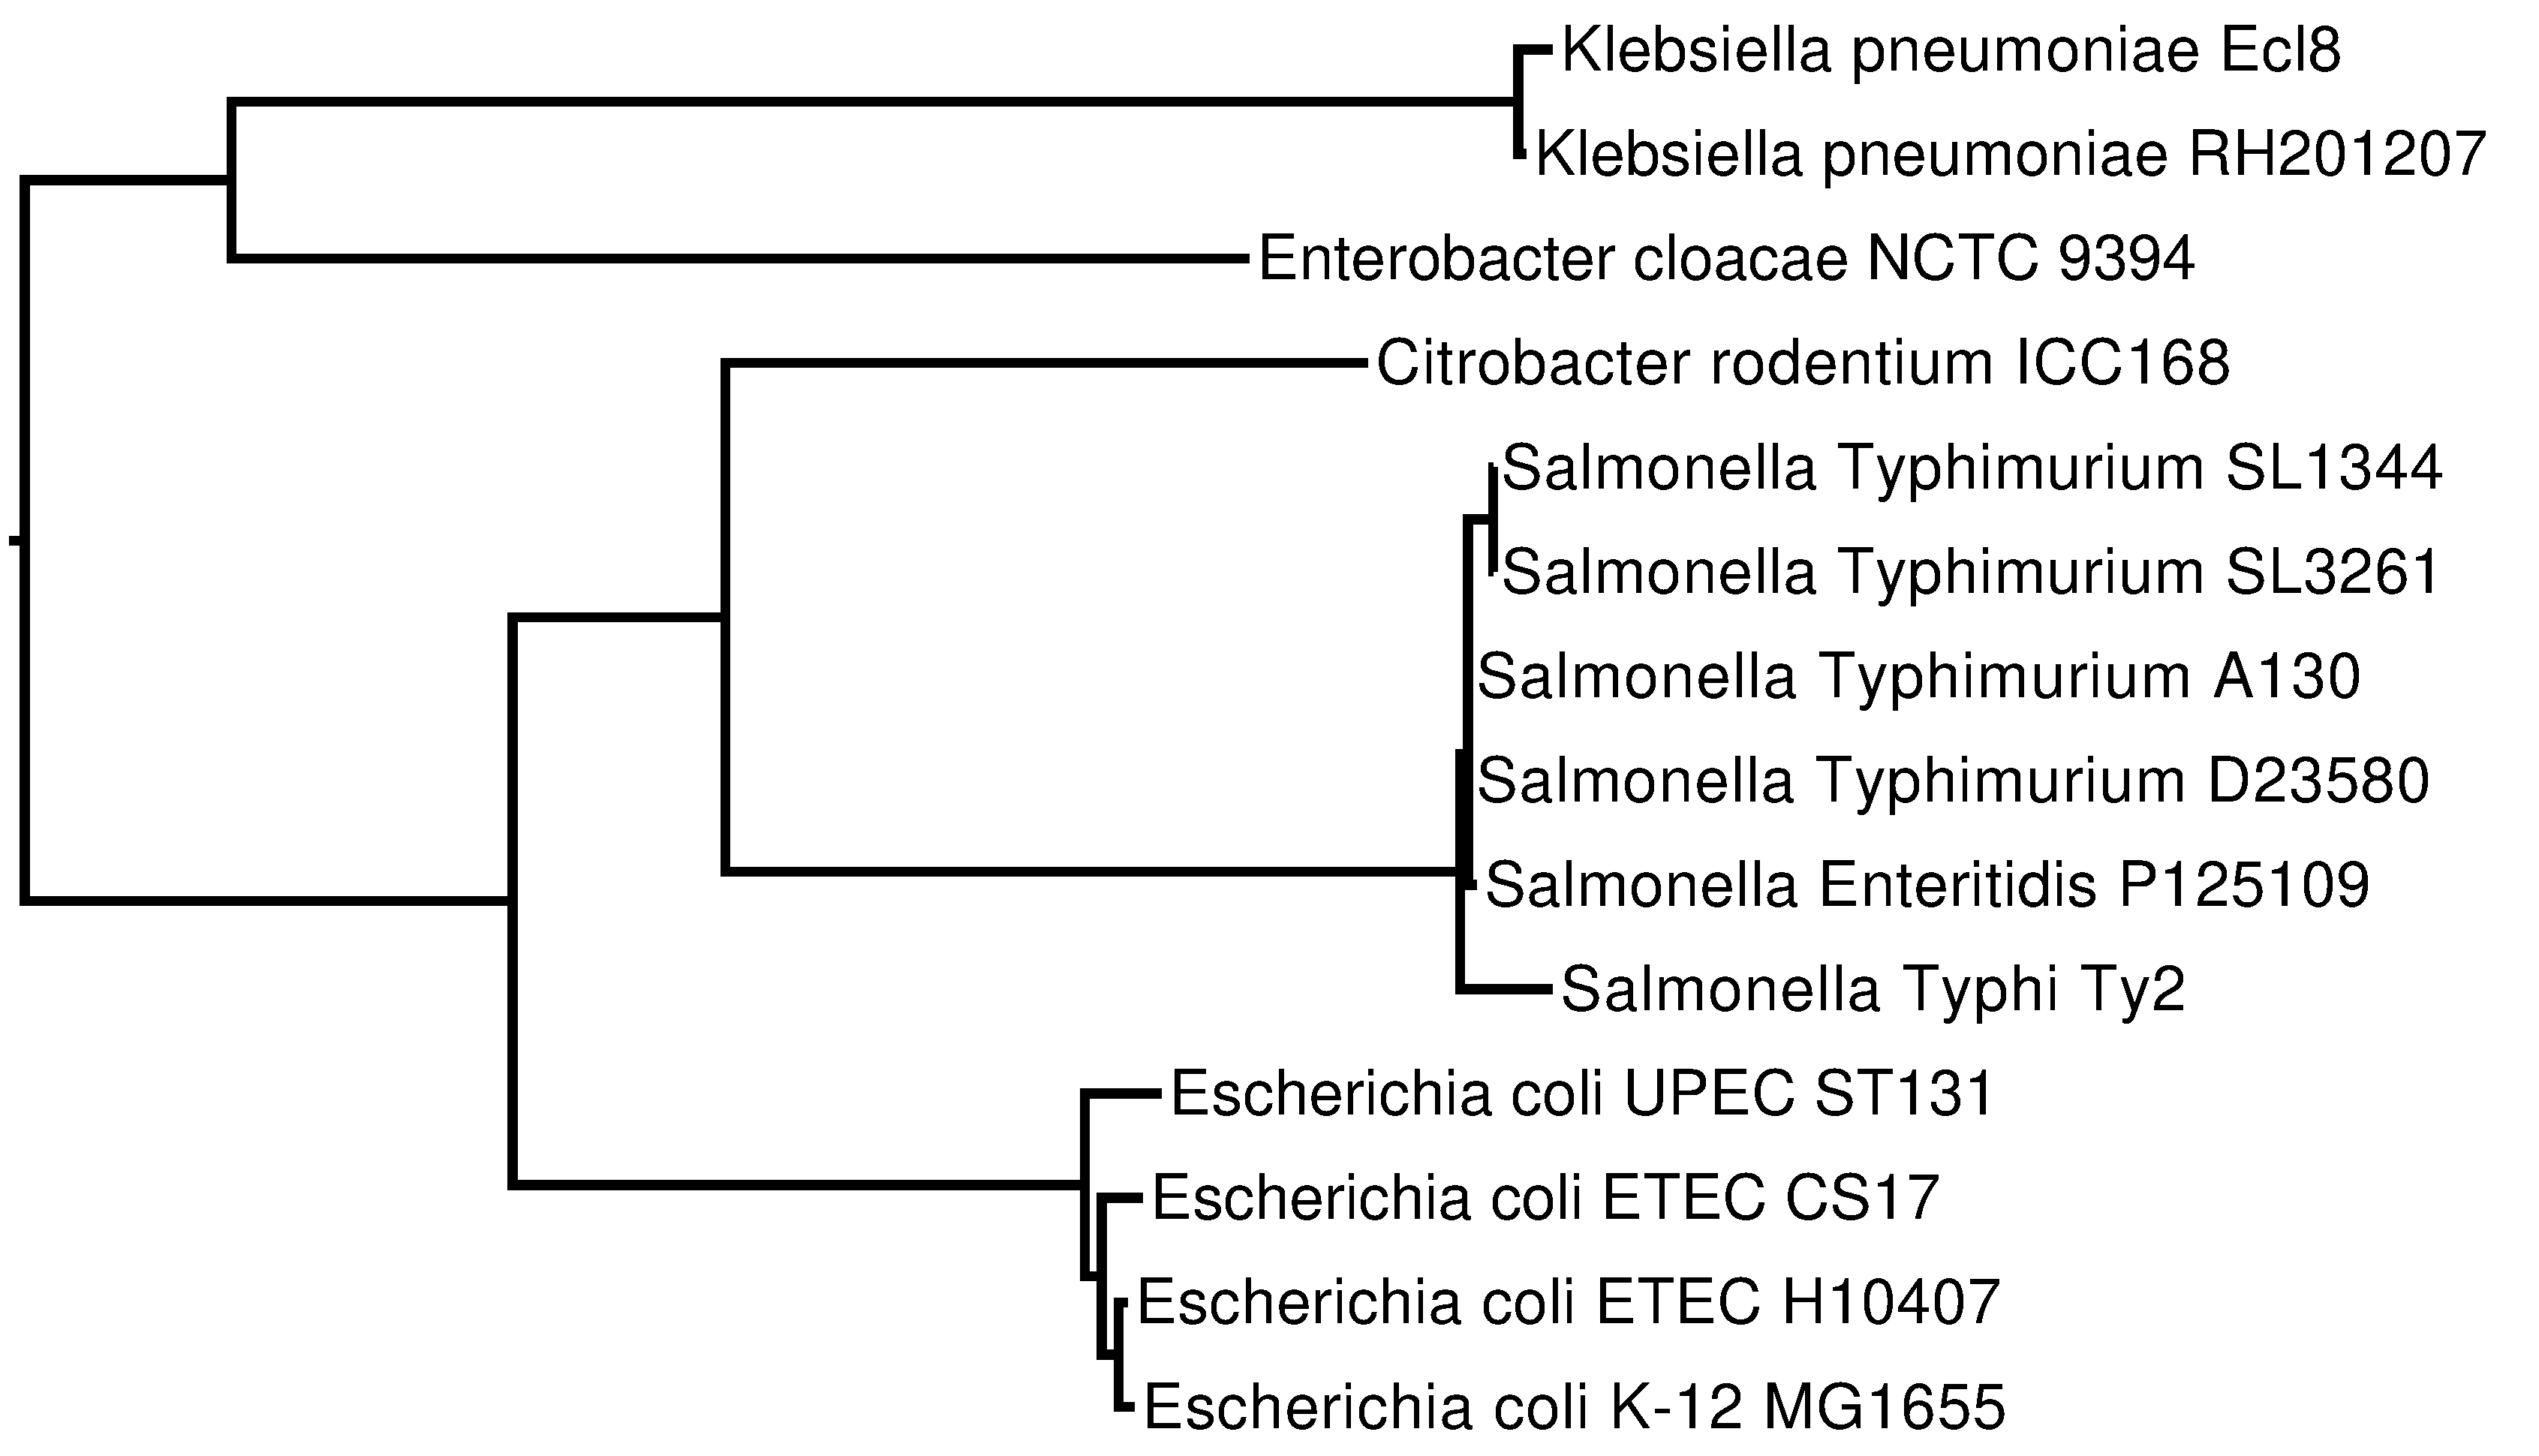
\includegraphics[scale=0.2]{phylosift-aa-raxmlbootstrap.pdf}
\caption{The species tree containing the 13 strains under study and Escherichia \textit{coli} K-12 MG1655 studied in Keio collection \cite{baba_construction_2006}. We have generated the tree by running RAxML \cite{stamatakis_raxml_2014} on Phylosift \cite{darling_phylosift:_2014} amino acid markers.}
\label{fig:species-tree}
\end{figure}

\section{Results and discussion}
Throughout time, species can gain or lose genes. We investigated if these gene gain and losses are related to the essentiality of the genes. In this section, we have first described the biases that can affect our study, and then evaluated the essentiality of genes and their conservation and the relationship between these two.

\subsection{Are there biases in transposon mutagenesis data?}
To evaluate the essentiality of a gene, the number of insertions within that gene was measured as explained in~\ref{sec:essentiality}. However, if the transposons are biased to specific regions in the genome, it results in false predictions and influences the accuracy of our analysis. Different articles have reported biases in transposon mutagenesis \cite{barquist_comparison_2013, rubin_essential_2015, kimura_nucleoid_2016}. We performed a detailed study of these biases. The biases that we have studied include: origin of replication bias, preferred insertion motif bias, and positional bias within genes.

%\subsection{Length bias}
%Short genes are less probable to be hit by transposons and so the genes that are very short might have no insertions. As a result, normalising the number of insertions by the length of the genes does not affect the essentiality level of these genes. 
%In Fig.\@ \ref{fig:length-bias} we have studied if the length of genes can influence their essentiality and we have found no correlation between length and insertion index in short genes. It seems that the insertion density in our experiment is high enough to make it possible for every gene to be hit by transposons.
%\begin{figure*}
%\centering
%\includegraphics[page=42, scale=0.3]{biases.pdf}
%\caption{The plot shows the lengths of the genes against their insertion indices. The red line shows the loess curve when the smoothness parameter is $0.2$.}
%\label{fig:length-bias}
%\end{figure*}

\subsubsection{Origin of replication bias}
One possible source of bias is the distance from origin of replication. When the bacteria are under replication during the transposn insertion process, there are more copies of the genes close to the origin of replication than the genes further away. This results in more insertions in the genes near the origin of replication which can influence the accuracy of our predictions. The other factor that can affect the results is if essential genes are clustered near the origin by nature. Rocha and Eduardo \cite{rocha_replication-related_2004} have shown that unlike highly expressed genes, essential genes are not enriched near the origin of replication. However, the essential genes are more frequent in the leading strand than the lagging one.

To study the bias towards the position of the genes, we plotted the insertion index for each gene versus the distance of the gene from the origin of replication normalised by the length of the genome in Fig.\@ \ref{fig:distance-bias}. The figure indicates that the insertion indices decrease when the genes are located further from the origin of replication.

\begin{figure*}
\centering
\begin{tabular}{c c c}
\includegraphics[page=2, scale=0.25]{biases.pdf}&
\includegraphics[page=5, scale=0.25]{biases.pdf}&
\includegraphics[page=8, scale=0.25]{biases.pdf}\\
\includegraphics[page=11, scale=0.25]{biases.pdf}&
\includegraphics[page=14, scale=0.25]{biases.pdf}&
\includegraphics[page=17, scale=0.25]{biases.pdf}\\
\includegraphics[page=20, scale=0.25]{biases.pdf}&
\includegraphics[page=23, scale=0.25]{biases.pdf}&
\includegraphics[page=26, scale=0.25]{biases.pdf}\\
\includegraphics[page=29, scale=0.25]{biases.pdf}&
\includegraphics[page=32, scale=0.25]{biases.pdf}&
\includegraphics[page=35, scale=0.25]{biases.pdf}\\
&\includegraphics[page=38, scale=0.25]{biases.pdf}&\\
\end{tabular}
\caption{The plots show the distance of the genes from DnaA gene normalised by the lengths of the genomes versus the insertion indices of the genes. The distance from DnaA gene has been calculated in both directions and then the minimum value has been used for distance. The red curves show the loess curve when the smoothness parameter is $0.2$.}
\label{fig:distance-bias}
\end{figure*}

\subsubsection{Preferred insertion motif bias}
Another concern while inferring essentiality from transposon mutagenesis data is that transposons are biased to certain compositions of nucleotides and high number of insertions in genes reflects the enrichment of the motifs that transposons are inclined to, instead of their essentiality level. For this, we used Weblogo~\cite{crooks_weblogo:_2004} to generate a logo from 10 nucleotides flanking the 100 top most frequent insertion sites in each genome. The results in Fig.\@  \ref{fig:logos} show a slight bias towards certain combinations of bases.

In addition, we investigated if the G-C content of genes can change the number of insertions by plotting the number of G-C bases in a gene normalised by the length of the gene versus insertion index (Fig.\@  \ref{fig:GC-bias}). As the figure shows, when G-C content is less than $40\%$, the insertion index is low, however when it is higher than $50\%$, the insertion index is almost constant. A possible reason for this phenomena is the association of A-T rich sequences and histone-like nucleotide structuring (H-NS) proteins, which reduces the insertions in A-T rich regions \cite{kimura_nucleoid_2016}. The other reason is that the genes with low G-C content are enriched in mobile genetic elements compared to the genes with average G-C content (Fig.\@ \ref{fig:gc-pval}) and this has caused seeing a different pattern of essentiality in that region.

\begin{itemize}
\item model H-NS binding sites? CGWTWHWww Lang et al (2007)
\item seems unlikely -- show bulk of genes are around 50\% G+C (add box-whisker plots to scatter diagrams?)
\item check Freed, Silander paper -- the missing piece of genome, was this low G+C? It is not mentioned in the paper.
\end{itemize}

\begin{figure*}
\begin{tabular}{c c}
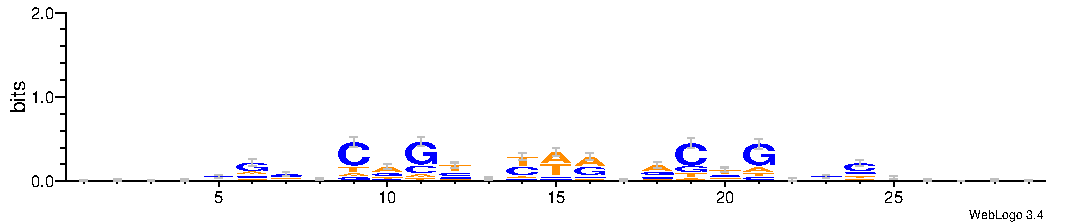
\includegraphics[scale=0.55]{100logo-bits.pdf}&
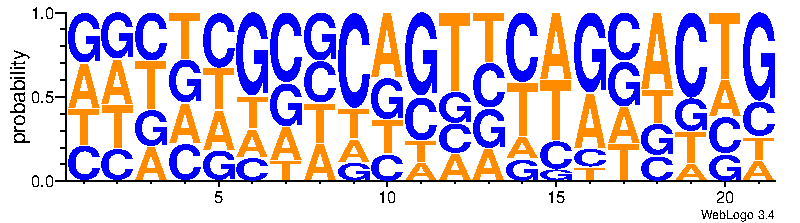
\includegraphics[scale=0.55]{100logo-prob.pdf}
\end{tabular}
\caption{Sequence logo plots generated using sequences from 10 nucleotides flanking the 100 top most frequent insertion sites from each genome. On the left the height of each character corresponds to a bit score for that character (i.e. $2-\sum f_a\times\log_2f_a-\frac{1}{\ln2}\times\frac{3}{2\times n}$, where $f_a$ is the relative frequency of base $a$ and $n$ is the number of sequences). To put it in simple words, the height of the set of characters shows how biased that position is and the height of each character shows the amount of bias towards that character. On the right the height of each character shows the relative frequency of that character.}
\label{fig:logos}
\end{figure*}

\begin{figure*}
\centering
\begin{tabular}{c c c}
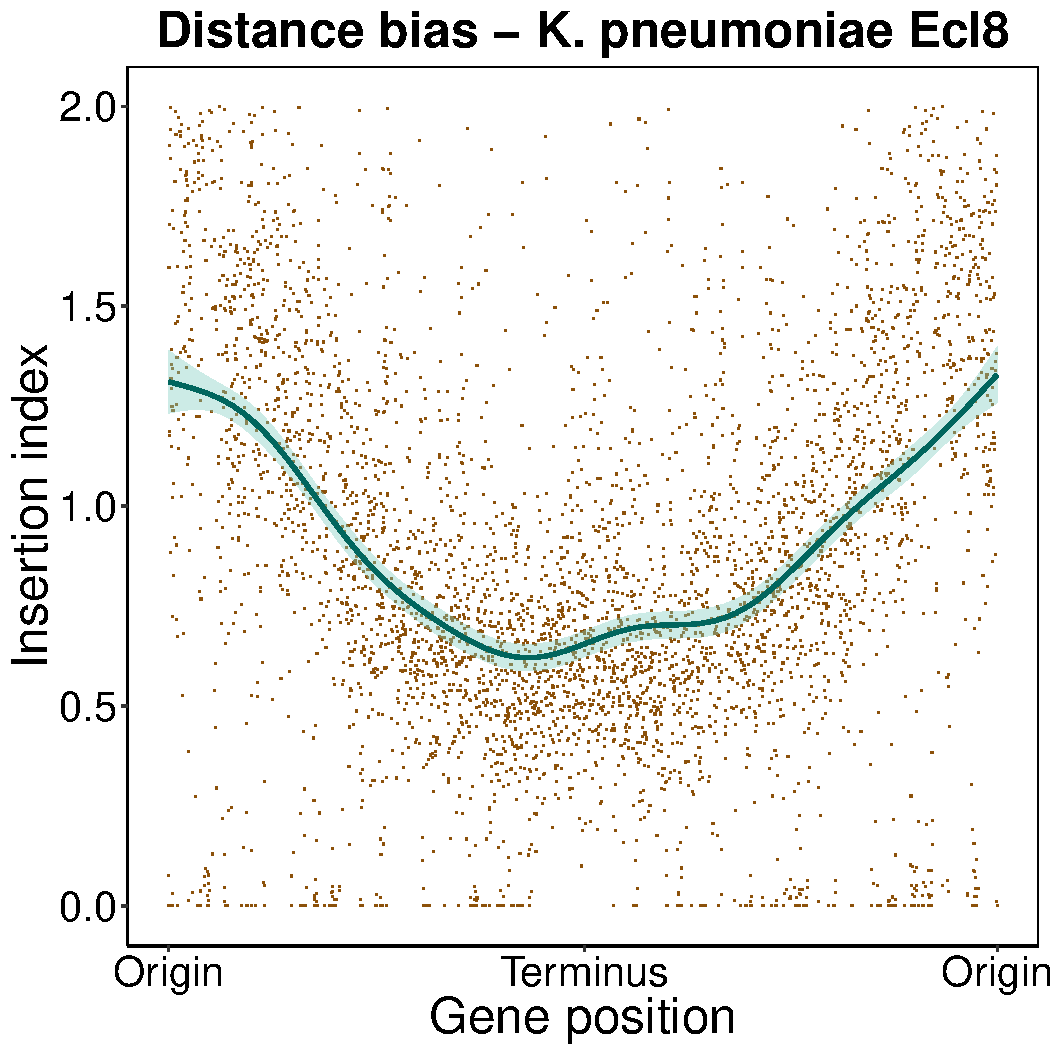
\includegraphics[page=1, scale=0.25]{biases.pdf}&
\includegraphics[page=4, scale=0.25]{biases.pdf}&
\includegraphics[page=7, scale=0.25]{biases.pdf}\\
\includegraphics[page=10, scale=0.25]{biases.pdf}&
\includegraphics[page=13, scale=0.25]{biases.pdf}&
\includegraphics[page=16, scale=0.25]{biases.pdf}\\
\includegraphics[page=19, scale=0.25]{biases.pdf}&
\includegraphics[page=22, scale=0.25]{biases.pdf}&
\includegraphics[page=25, scale=0.25]{biases.pdf}\\
\includegraphics[page=28, scale=0.25]{biases.pdf}&
\includegraphics[page=31, scale=0.25]{biases.pdf}&
\includegraphics[page=34, scale=0.25]{biases.pdf}\\
\includegraphics[page=37, scale=0.25]{biases.pdf}&&
\includegraphics[page=40, scale=0.25]{biases.pdf}\\
\end{tabular}
\caption{The plots show the ratio of G-C bases in the genes normalised by the lengths of the genes against their insertion indices. The red curves show the loess curve when the smoothness parameter is $0.2$.}
\label{fig:GC-bias}
\end{figure*}

\begin{figure*}
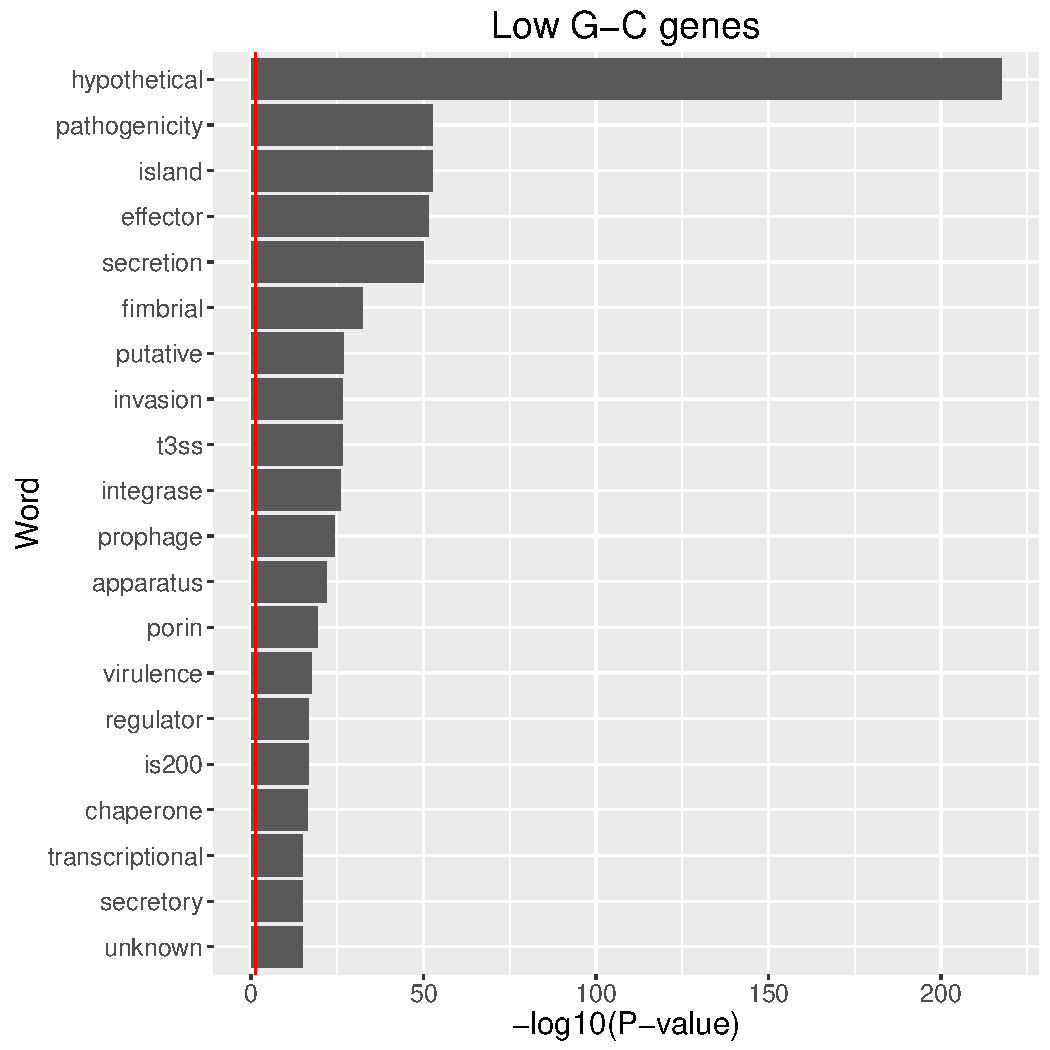
\includegraphics[scale=0.55]{lowgc-pval.pdf}
\caption{Word enrichment analysis for low G-C genes compared to genes with interquartile G-C level. The red line shows P-value = 0.05. The P-values have been calculated using Fisher's exact test and corrected using Benjamini-Hochberg-Yekutieli.}
\label{fig:gc-pval}
\end{figure*}

\subsubsection{Positional bias within genes}
The other question that we tried to answer was whether insertions are tolerated in some regions in a gene. For example, can essential genes tolerate insertions at their 3' end without losing their funtionality? To address this question, we divided every gene into percentiles and calculated the mean insertion index for each percentile. Fig.\@ \ref{fig:insertion-position-bias} shows almost no bias towards any location when considering all genes together. We also studied the bias in three of the groups defined in Section~\ref{sec:essentiality}: essential genes, non-essential genes, and beneficial losses. The results imply that the number of insertions in the internal region of the essential genes is outnumbered by the number of insertions in the 5' and 3' ends while it is the opposite in beneficial losses. The case for the non-essential genes is similar to all genes. High number of insertions at the 3' end of essential genes implies that the functional part of the genes are located before the insertions. On the other hand, high number of insertions at the 5' end of the essential genes indicates there might be alternative start codons in the 5' end or it might be because of alignment errors. \textcolor{red}{\{To be tested\}}

\begin{figure*}
\begin{tabular}{c c}
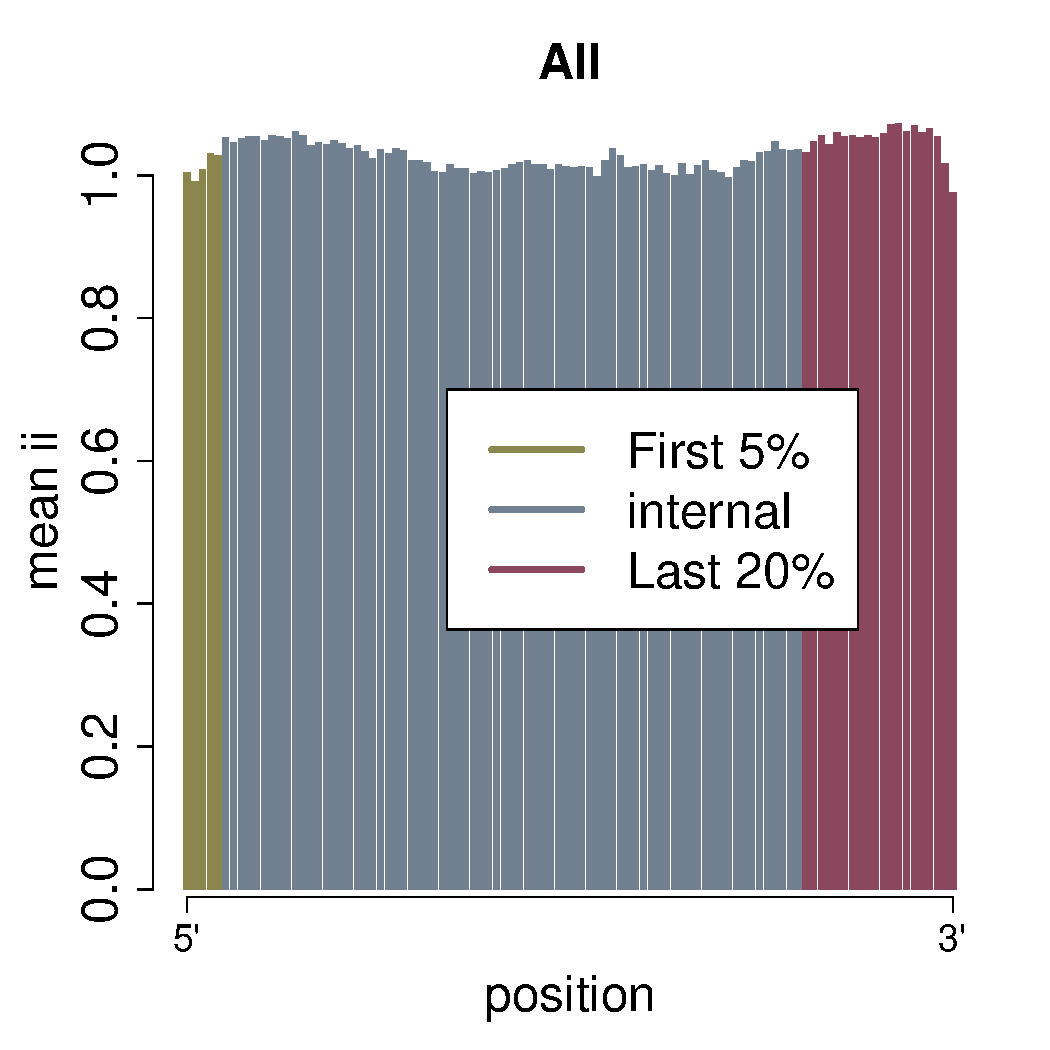
\includegraphics[scale=0.4, page=1]{insertion-position-bias.pdf}&
\includegraphics[scale=0.4, page=2]{insertion-position-bias.pdf}\\
\includegraphics[scale=0.4, page=3]{insertion-position-bias.pdf}&
\includegraphics[scale=0.4, page=4]{insertion-position-bias.pdf}
\end{tabular}
\caption{The plots show the average insertion index in the percentiles of all genes (top left), essential genes (top right), non-essential genes (bottom left), and beneficial losses (bottom right). The genes are divided into 3 segments: 5\% of
the genes on the 5' end, 20\% of the genes on the 3' end, and the rest in the middle. These are shown by khaki, slate gray, and violet red respectively.}
\label{fig:insertion-position-bias}
\end{figure*}

%\begin{itemize}
%\item There is a bias towards the position of the gene (Fig.~\ref{fig:distance-bias}).
%\item There is a negligible bias towards certain motifs (Fig.~\ref{fig:logos})
%\item The G-C bias needs to be studied further (Fig.~\ref{fig:GC-bias})
%\item The number of insertions on the 3' and 5' ends is more than the internal region in essential genes and less than the internal region in beneficial losses. (Fig.~\ref{fig:insertion-position-bias})
%\end{itemize}
\subsection{Essentiality and conservation}
Essential genes are needed for the growth of organisms. Because of that, one might think that essential genes should not be lost in a short period of time throughout evolution, unless they are no longer needed in new organisms or they are replaced by new pathways. Therefore, it is expected that most of the essential genes are conserved in different organisms from the same family. We have tested this idea by comparing the essentiality and conservation of genes in Enterobacteriaceae family.


\subsubsection{Gene classes}
%We needed to cluster sets of orthologous genes in our strains to study the conservation of essentiality. Plenty of methods are proposed for this purpose. Altenhoff et al.\@ have compared 15 of these methods \cite{altenhoff_standardized_2016} and shown that Hieranoid \cite{schreiber_hieranoid:_2013} is among three methods that keep a balance between precision and recall. We have used Hieranoid to cluster the sets of orthologous genes. In addition, we intended to study the essentiality of genes in paralogous genes. For this, we have developed a program that clusters all homologous genes using Jackhmmer from HMMER3 package \cite{mistry_challenges_2013}.
In order to study the relationship between essentiality and conservation, we needed to evaluate the essentiality and conservation of genes. For this, we divided the genes into different levels of essentiality (essential genes, ambiguous, non-essential genes, beneficial losses). We first normalised the biases that exist in the data using the method explained in Section~\ref{sec:biascorrection} and then defined the essentiality level of genes using the method explained in Section~\ref{sec:essentiality}. Moreover, we grouped the genes into different classes of conservation (genus specific, single copy, multi-copy) using the method explaind in Section~\ref{sec:conservationclasses}.

The results for comparing four levels of essentiality and three classes of conservation are depicted in Fig.\@ \ref{fig:iidist}. The high number of single copy genes in essential level, indicates that there is a set of essential genes in Enterobacteriaceae that are conserved and inclined to keep their essentiality. However, the relatively high number of essential genes in genus specific class implies that each genus has a set of essential genes that makes it distinct. The figure also shows that beneficial losses are over represented in genus specific class. Therefore, beneficial losses are mostly recent genes that the organism tends to lose in the long run. Besides, most of the multi-copy clusters are non-essential and there are only a few multi-copy clusters that are essential. This can be explained by the redundancy that genes can keep even after $\sim100$ million years \cite{dean_pervasive_2008}. In the presence of two redundant variations of one gene, if we knock out one copy by transposon mutagenesis, the other copy compensates and the organism can still survive.

\begin{figure}
\centering
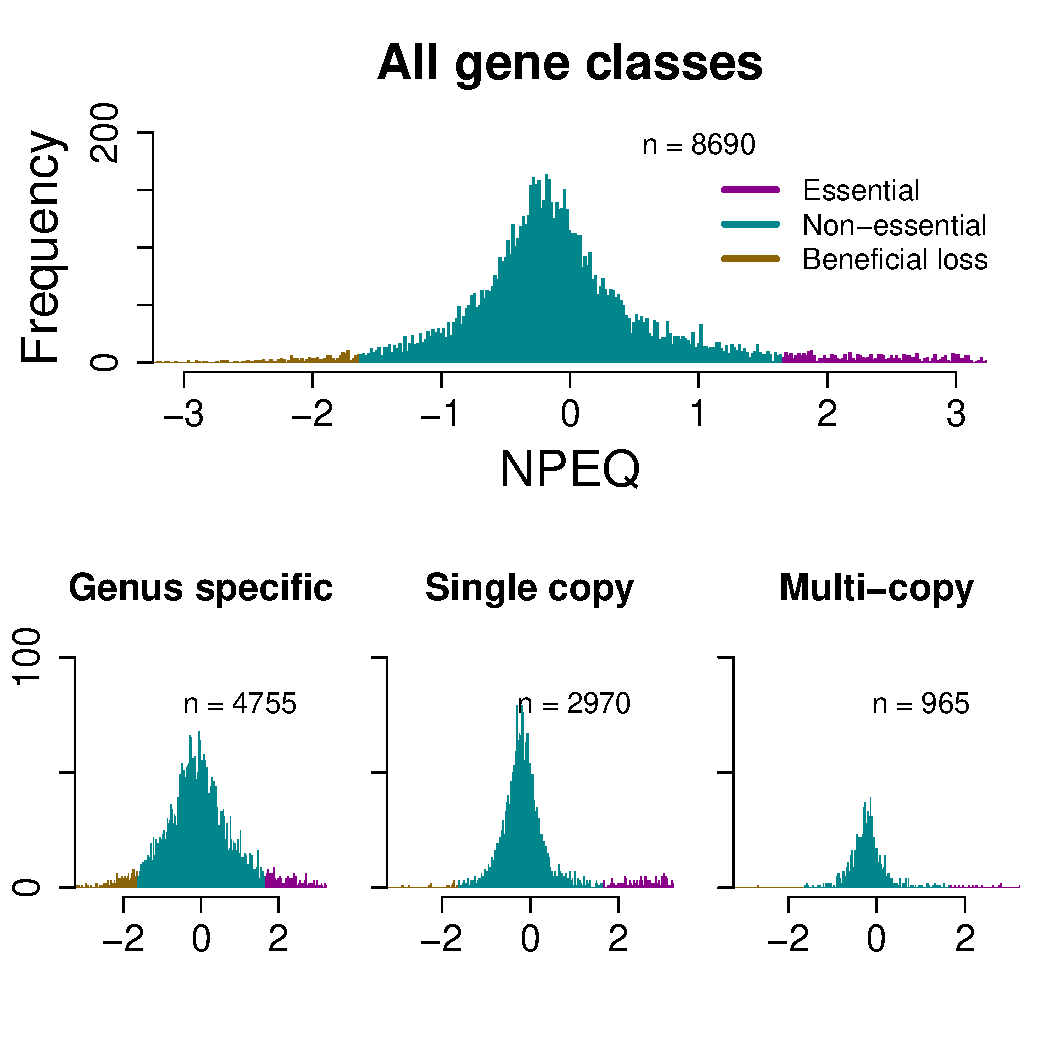
\includegraphics[scale=0.5]{cluster-essentiality.pdf}
\caption{The genes have been clustered into orthologous groups using Hieranoid and paralogous groups using Jackhmmer and divided into 3 groups: genus specific, single copy, and multi-copy genes. Then, the essentiality of the clusters has been defined using the insertion indices of the genes in the clusters. The figure shows that most of the essential genes are in single copy group, while most of the beneficial losses are genus-specific.}
\label{fig:iidist}
\end{figure}

To study which functions are enriched in each class of essentiality, we gathered the descriptions of genes from their embl files. Then, we counted the repeat number of each word for the genes in each class and the genes that do not belong to that class and the number of all other words in these two groups and used a Fisher's exact test to calculate P-values. The P-values are then corrected using Benjamini-Hochberg-Yekutieli procedure. Fig.\@ \ref{fig:essentiality-pval} shows the top 20 enriched words for each essentiality class. The results show an enrichment of the genes related to replication, transcription, translation, division, and rod shape determining proteins in essential class. The non-essential genes are mostly membrane associated proteins, flagellar proteins, ATPase, and DNA repair proteins. Beneficial losses are enriched in transposase enzymes, putative and hypothetical proteins, and mobile elements. Beneficial losses also contain many fimbrial proteins which probably has occurred because these proteins are not needed in a rich lab medium \textcolor{red}{\{TRUE?\}}.
%We have done a word enrichment analysis on the description of the beneficial losses in Fig.\@ \ref{fig:essentiality-pval}. It shows that most of the beneficial losses are mobile elements. Most of these mobile elements are not included in KEGG database.

We also conducted a pathway enrichment analysis for these three groups. For this, we downloaded pathway datasets for strains that were available in KEGG database. This includes pathways for Cirobacter rodentium ICC168, Salmonella Enteritidis P125109, Enterobacter cloacae NCTC 9394, Salmonella Typhimurium D23580, Escherichia coli ETEC H10407, Salmonella Typhimurium SL1344, Escherichia coli K-12 MG1655, and Salmonella Typhi Ty2. Then we merged these databases and used the hypergeometric test to find which pathways were enriched in each essentiality class. Finally, we corrected the P-values using Benjamini-Hochberg-Yekutieli. The results (Fig.\@ \ref{fig:essentiality-pathway}) suggest similar results to the enrichment analysis that we had done on the description of the genes. However, as mobile genetic elements are not stored in KEGG database, the pathway enrichment analysis does not show the enrichment of mobile genetic elements in beneficial-losses.

\begin{figure*}
\centering
\begin{tabular}{c c}
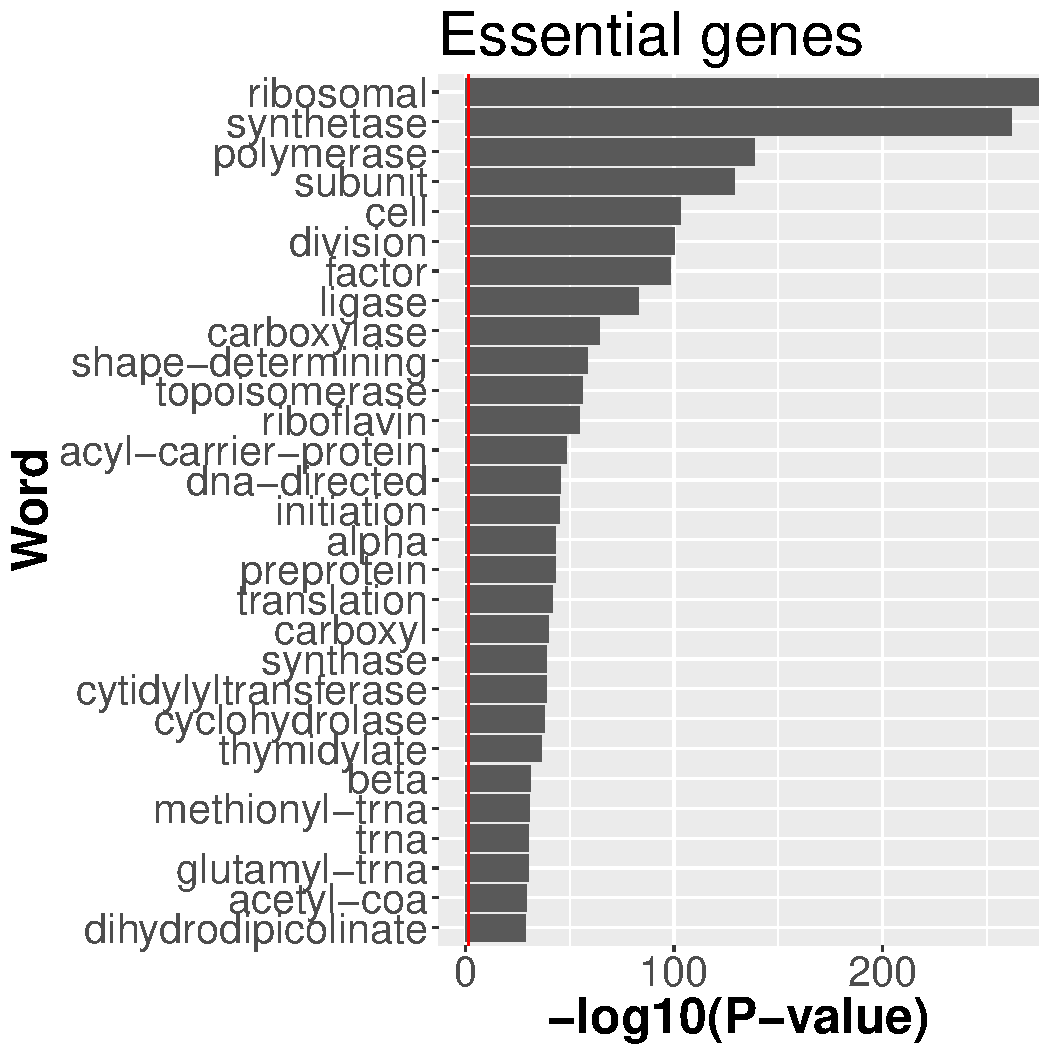
\includegraphics[scale=0.4]{essential-pval.pdf}&
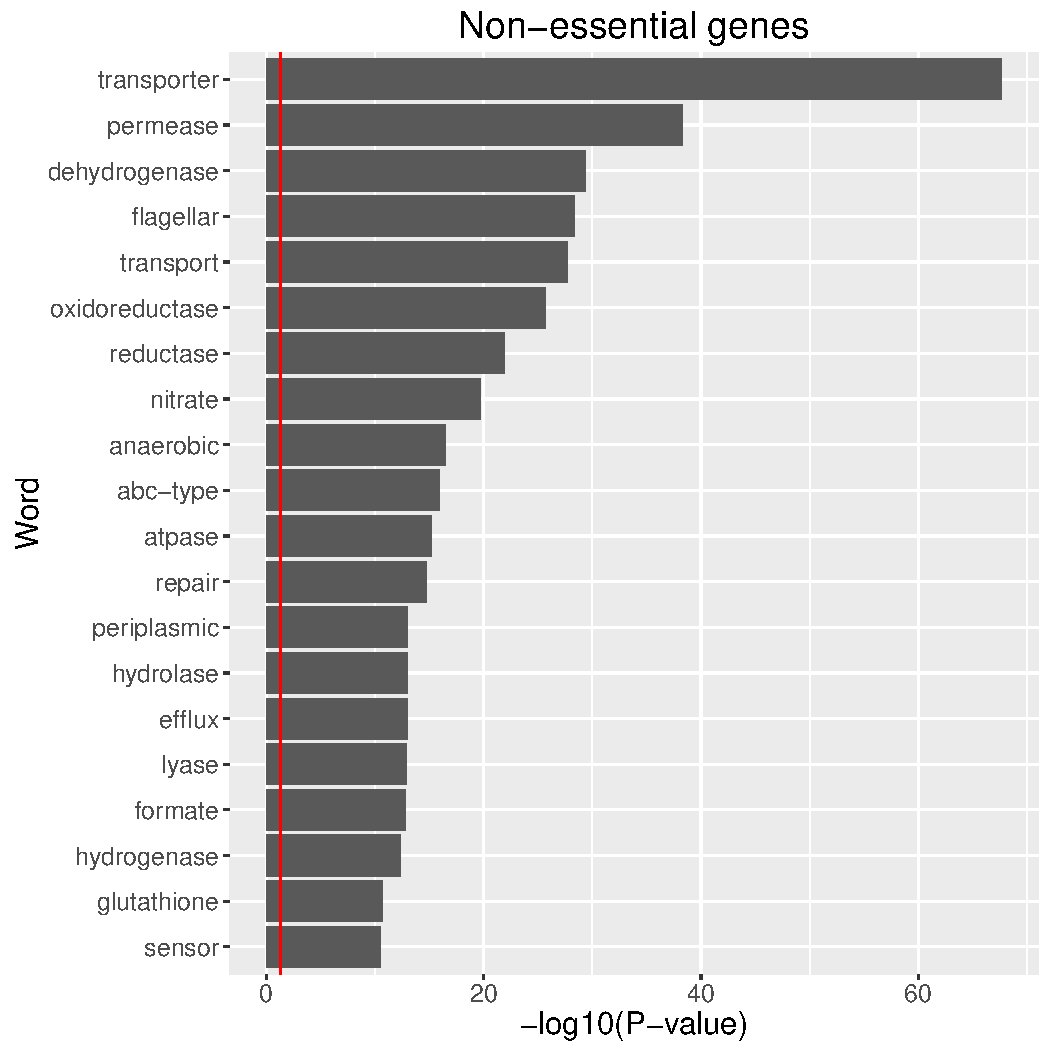
\includegraphics[scale=0.4]{non-essential-pval.pdf}\\
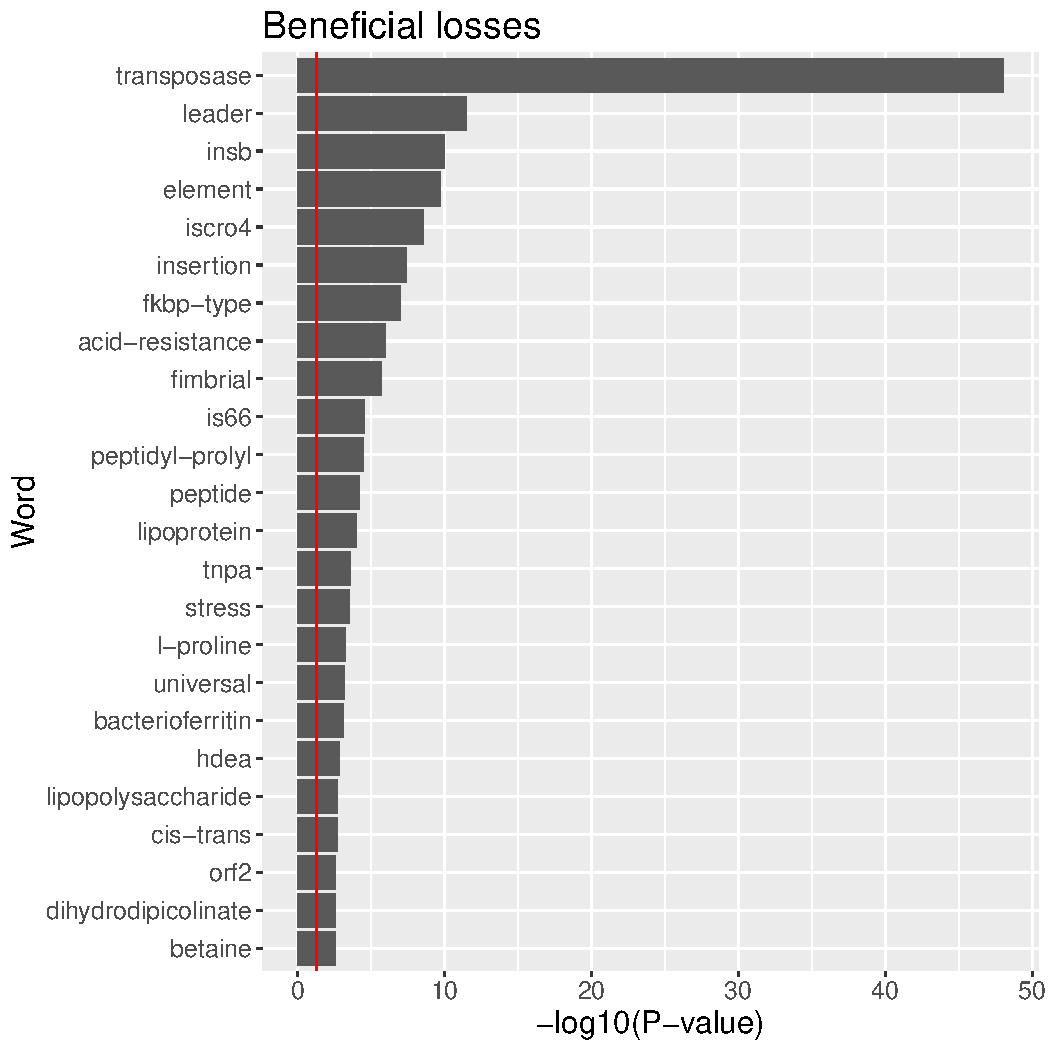
\includegraphics[scale=0.4]{beneficialloss-pval.pdf}&
\end{tabular}
\caption{Word enrichment analysis for essential genes, non-essential genes, and beneficial losses compared to other genes. The red line shows P-value = 0.05. The P-values have been calculated using Fisher's exact test and then corrected using Benjamini-Hochberg-Yekutieli procedure.}
\label{fig:essentiality-pval}
\end{figure*}

\begin{figure*}
\centering
\begin{tabular}{c c}
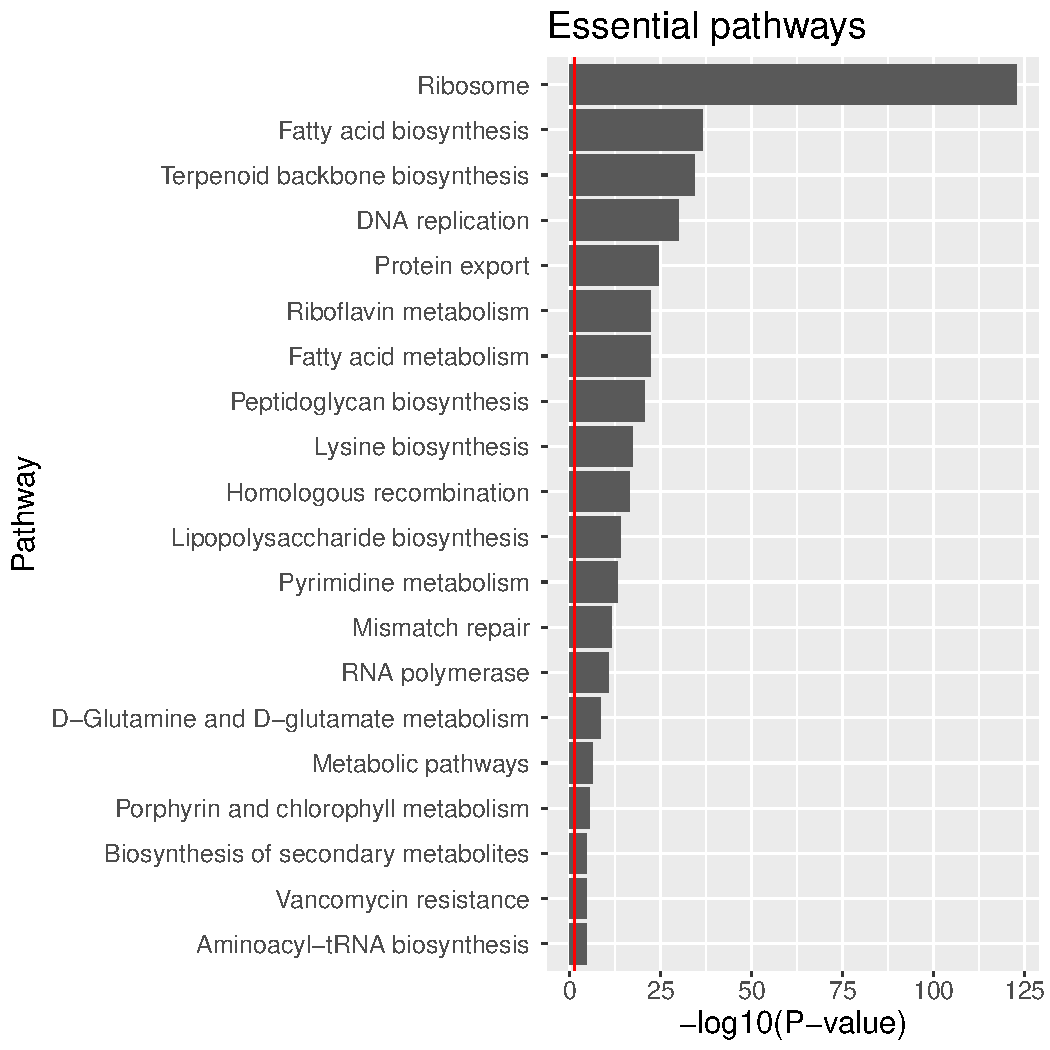
\includegraphics[scale=0.4]{essential-pathways.pdf}&
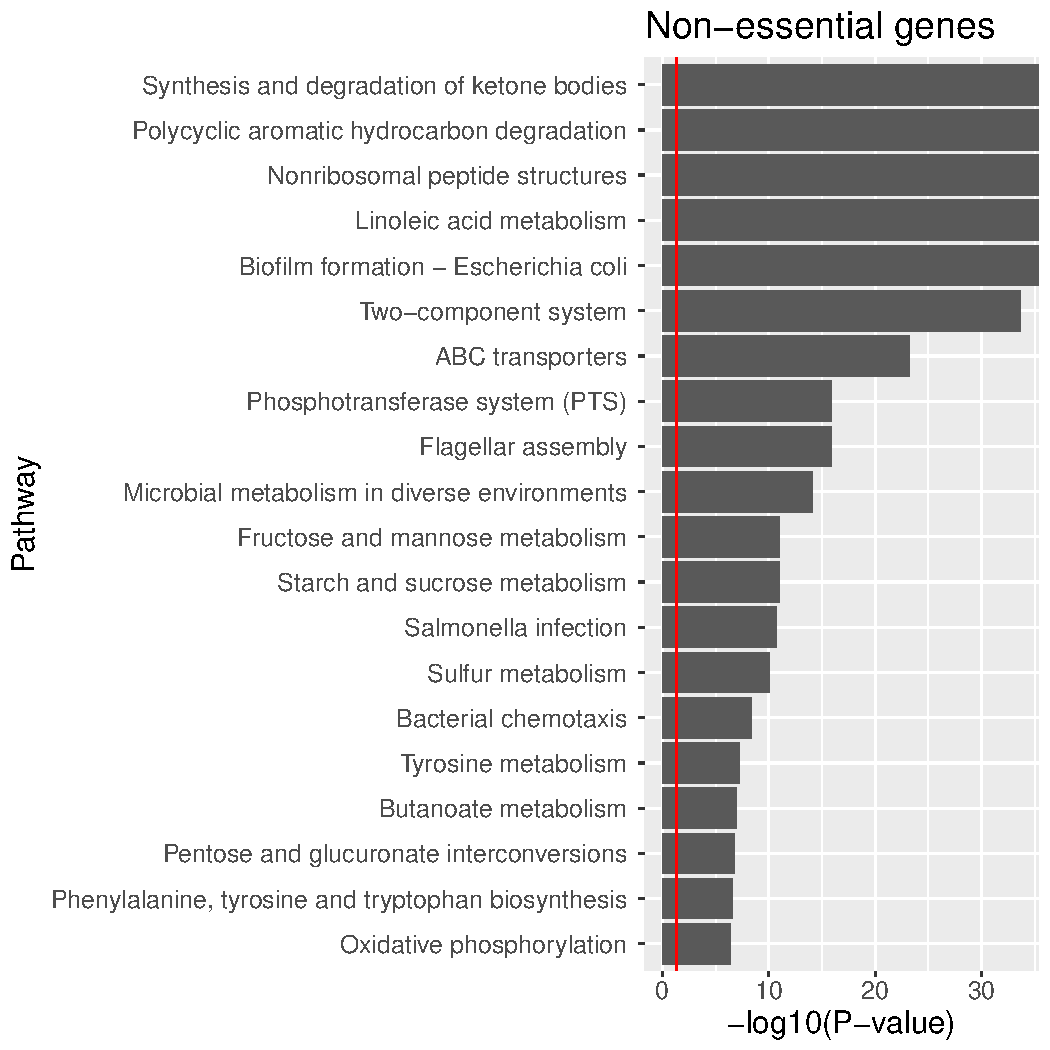
\includegraphics[scale=0.4]{non-essential-pathways.pdf}\\
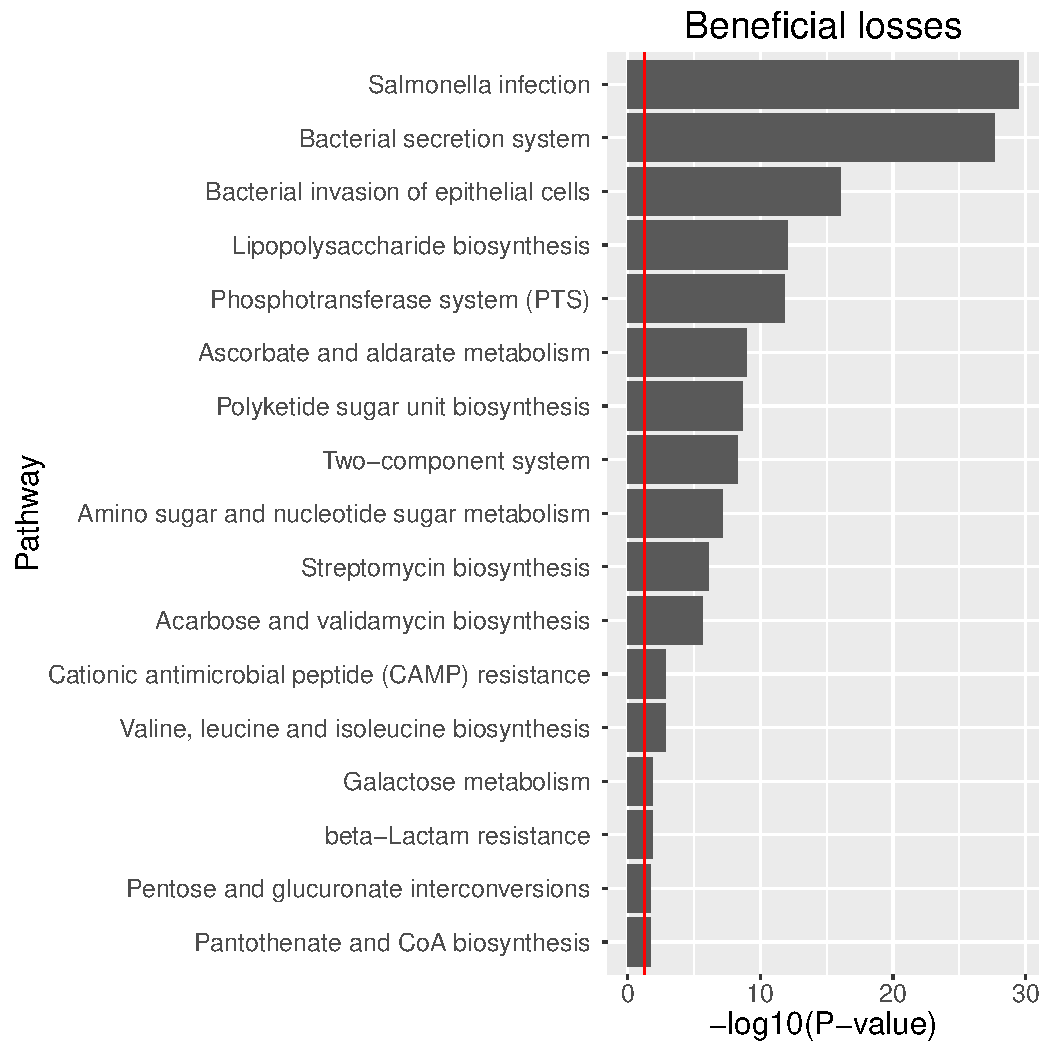
\includegraphics[scale=0.4]{beneficialloss-pathways.pdf}&
\end{tabular}
\caption{Pathway enrichment analysis for beneficial losses, essential genes, and non-essential genes compared to other genes. The red line shows P-value = 0.05. The P-values are calculated using hypergeometric test and then corrected using Benjamini-Hochberg-Yekutieli procedure.}
\label{fig:essentiality-pathway}
\end{figure*}

\subsubsection{The evolution of essentiality}
%In order to test if the essentiality of genes follows a tree-like trend we have gathered all the genes that are copied once per genome and made a matrix with rows showing genomes and columns showing genes. If a gene is essential in a genome, its corresponding cell in the matrix has value 1 and 0 otherwise. Then we have used the Bray-Curtis distance to generate a distance matrix for the species under study. Finally, a tree has been generated using PHYLIP Neighbor. The resulting tree is not similar to the species tree.
%
%\begin{figure}
%\centering
%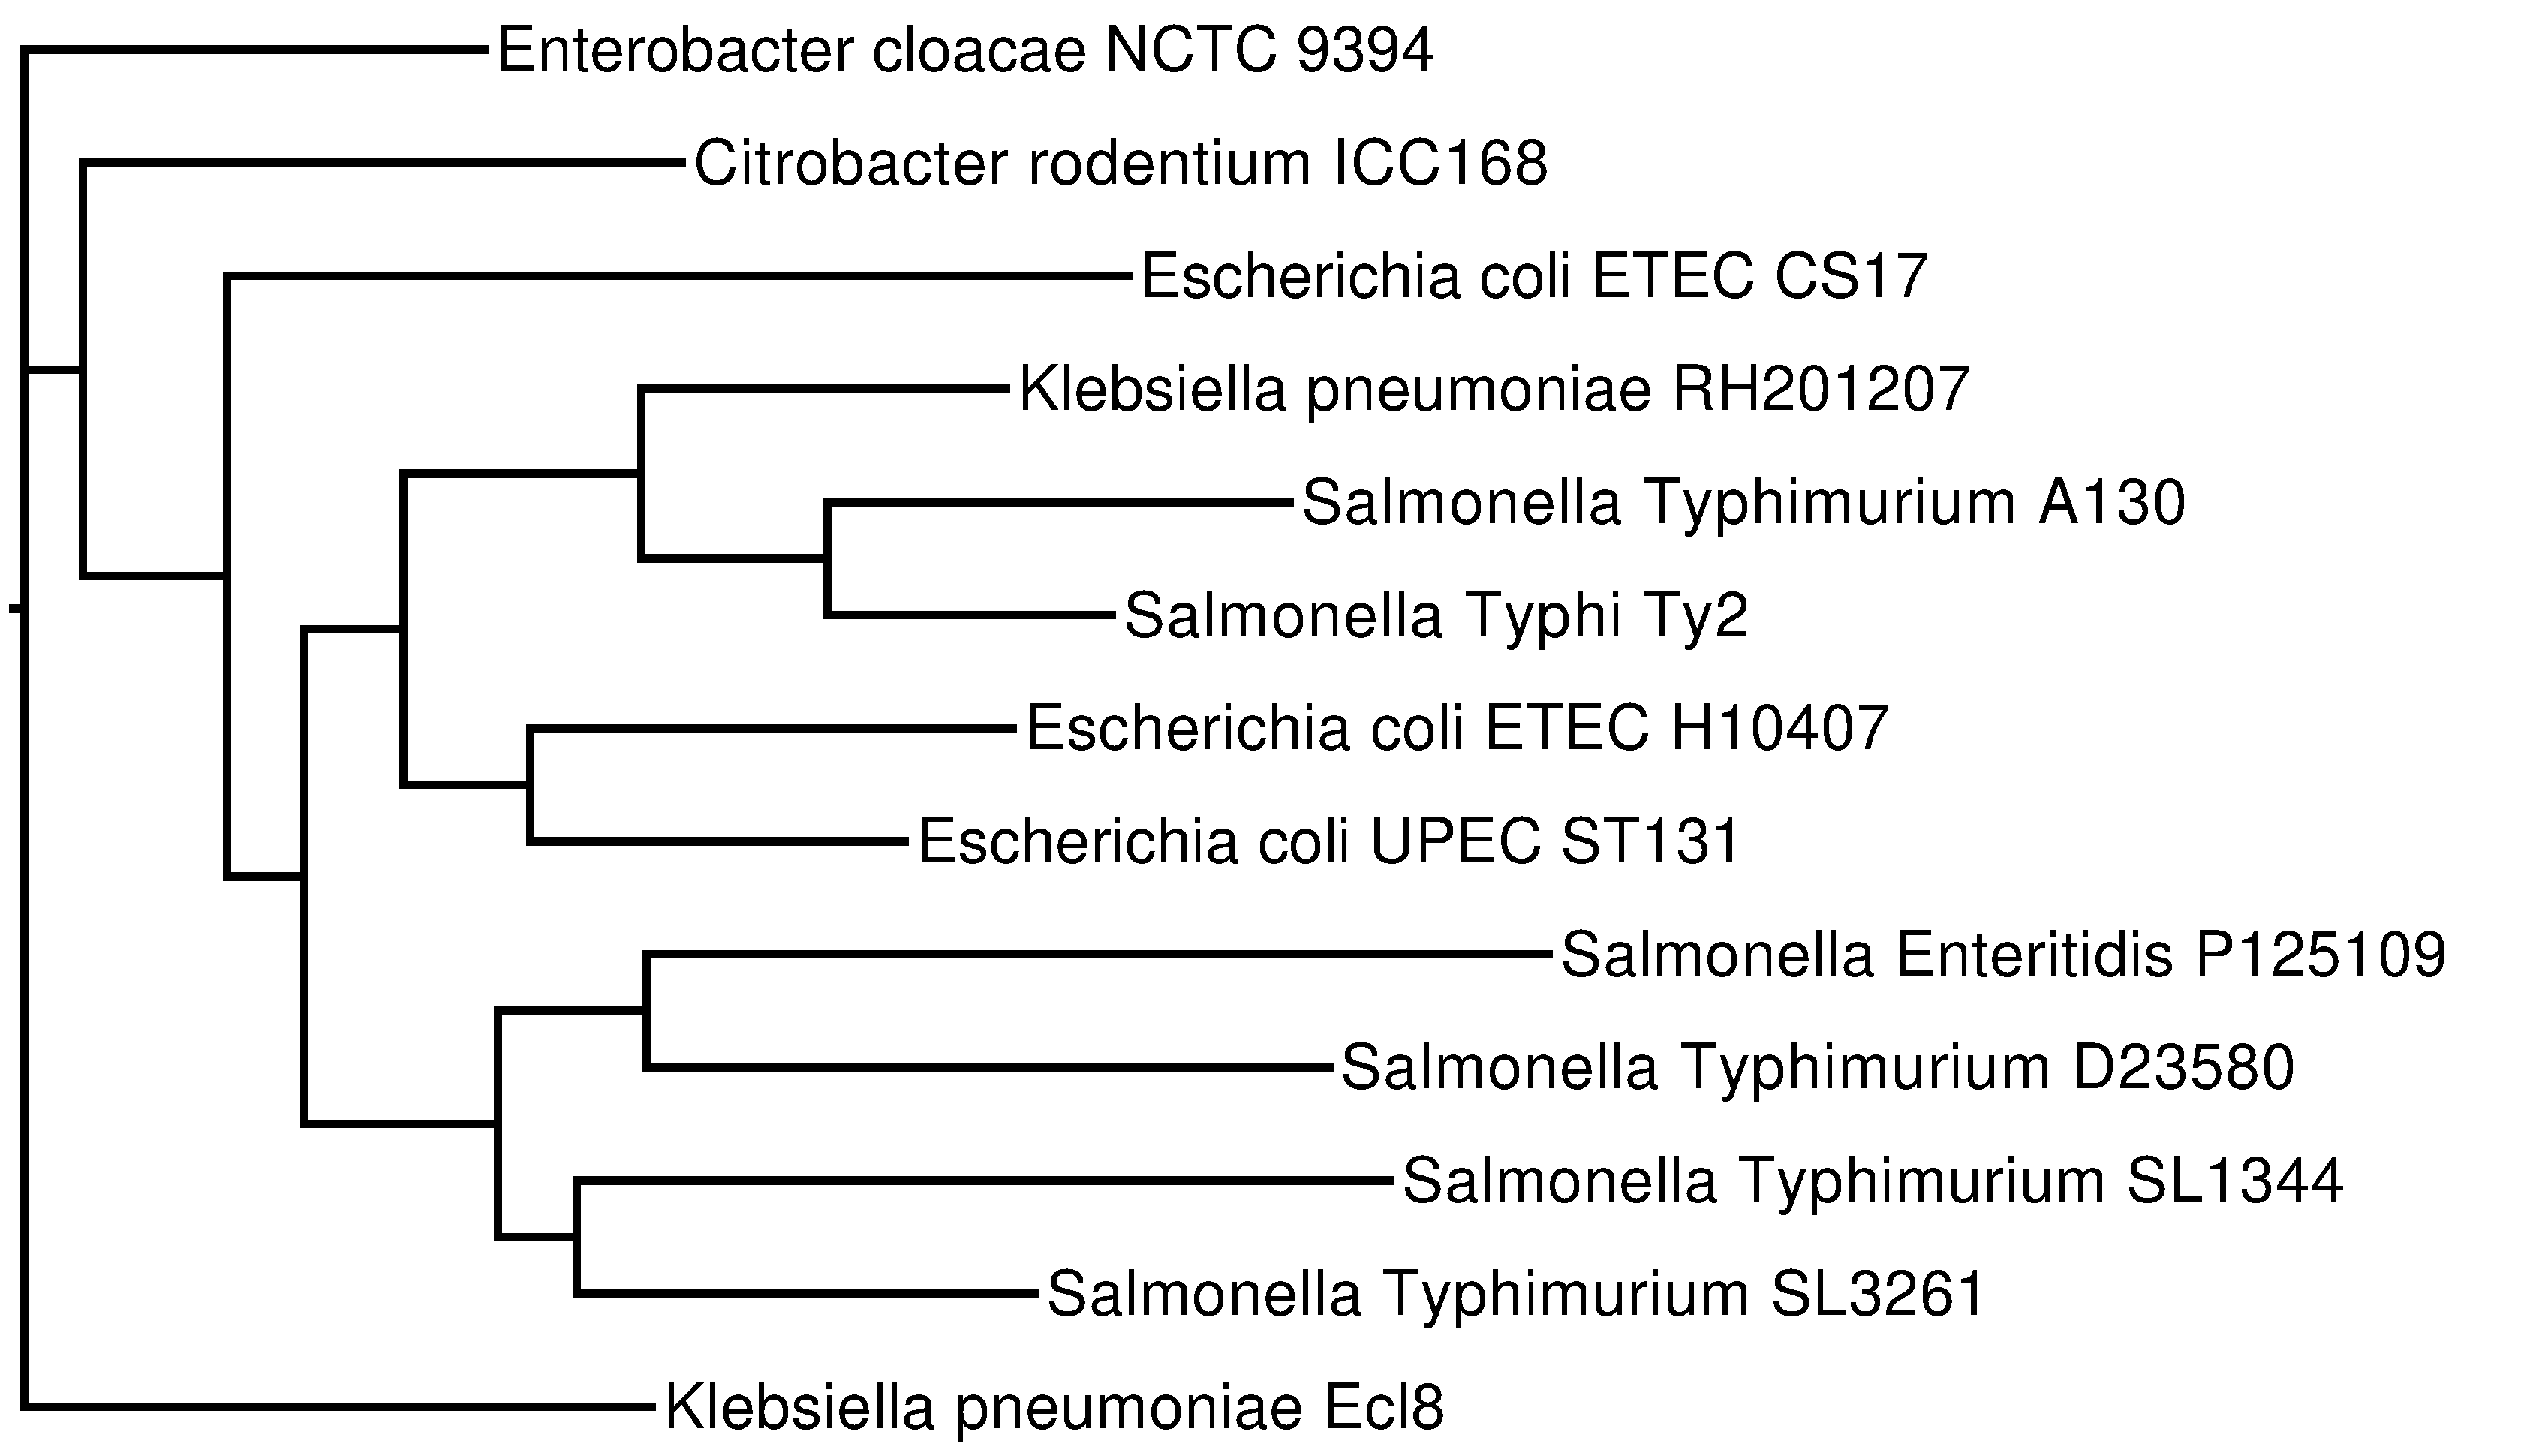
\includegraphics[scale=0.2]{neighbor-joining-essentiality-tree.pdf}
%\caption{The tree is generated from all the genes that are copied only once per genome. We have made a binary matrix from the essentiality of these genes. Then, we have generated a distance matrix from these values using Bray-Curtis distance and plotted a phylogenetic tree using PHYLIP Neighbor which uses a neighbour joining method.}
%\label{fig:neighborjoining}
%\end{figure}

In this section, we have counted the genes that are essential and conserved at each level of the phylogenetic tree. We were interested to see if the trend of the essentiality variation between different organisms is in agreement with the phylogenetic tree. In other words, we have tested if organisms close together have more essential genes in common than organisms that have separated earlier in the phylogenetic tree.

We needed to cluster sets of orthologous genes in the bacteria that we were studying. Homologous clusters introduced in ~\ref{sec:conservationclasses} were not useful for this purpose as sets of paralogous genes with different essentiality levels can make essentiality inference ambiguous. Plenty of methods are proposed for this purpose. Altenhoff et al.\@ have compared 15 of these methods \cite{altenhoff_standardized_2016} and shown that Hieranoid \cite{schreiber_hieranoid:_2013} is among three methods that keep a balance between precision and recall. We used Hieranoid for clustering orthologous genes.

In order to test if the essentiality of genes follows a tree-like trend, we compared the number of genes that were conserved in different bacteria in our study and the number of genes that were essential in these bacteria. The genes that are conserved in all bacteria being studied are called core genes and the genes that are conserved and essential are called core essential genes. We counted the number of genes that were core between every combination of bacteria, and the number of core essential genes between those combinations. We used UpSetR package \cite{conway_upsetr:_2016} in R to visualise the results in Fig.\@ \ref{fig:upsetr}. As shown in the figures, among 1908 genes that are core between all the bacteria under study, only 184 are core essential. We looked at subsets of the genes that were core essential (core) in every combination of our bacterial strains to see whether they were phylogenetically informative or not. A phylogenetically informative subset is a subset that is core essential (core) in two or more bacteria but not in all bacteria. We have marked the phylogenetically informative sets of genes with ticks and the uninformative ones with crosses. The results propose that although conservation of genes follows a tree-like trend with many phylogenetically informative sets of genes with high cardinality, the essentiality does not show a tree-like signal and most of the large sets of core essential genes belong to only one bacteria. We believe this is due to the small number of essential genes. Each bacterium has about 300 to 500 essential genes among which 184 is core essential between all bacteria. A portion of the remaining essential genes are specific to each bacterium and many are shared between all bacteria except one. The number of remaining essential genes is so low that causes the essentiality trend not to be tree-like. Furthermore, some of the predicted essential genes might be artefacts of transposon mutagenesis method.

\begin{figure*}
\centering
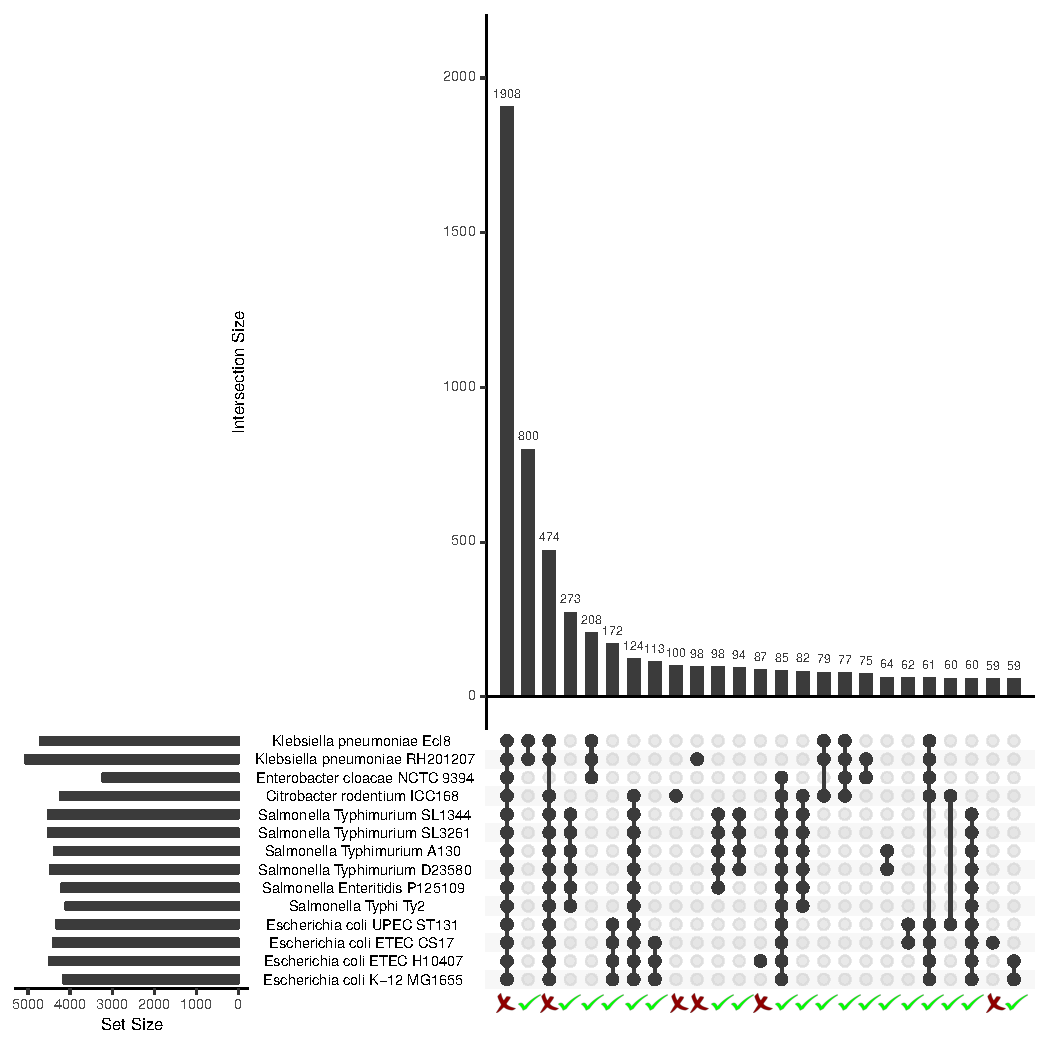
\includegraphics[scale=0.6]{upsetr1-edited.pdf}\\
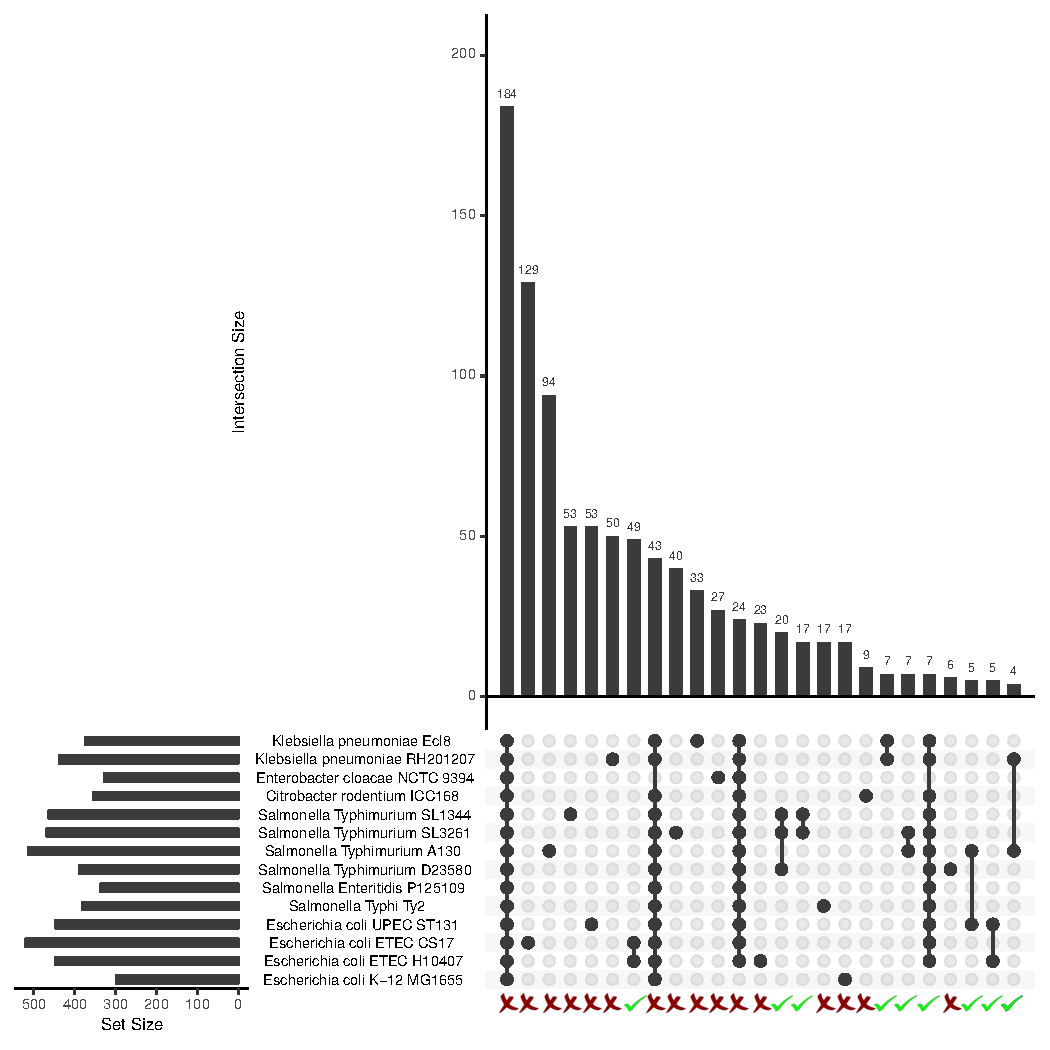
\includegraphics[scale=0.6]{upsetr2-edited.pdf}
\caption{The first figure shows the number of core genes between each group of species and the second figure shows the number of core essential genes. The bars show the number of genes that are core between the strains marked with black circles. The tick marks show phylogenetically informative columns and the cross marks show non-informative columns.}
\label{fig:upsetr}
\end{figure*}

To further study the trend of essentiality changes, we looked at different levels in the species tree and calculated the ratio of the number of core essential genes to the number of core genes in each level. We used three different methods for inferring core genes and core essential genes. These methods are explained in Section~\ref{sec:core}. The numbers predicted using these three methods are shown in Fig.\@ \ref{fig:annotated-speciestree}. As this figure shows, the ratio between core essential and core genes is almost constant using the intersection and dollo method; however, this ratio increases as we go higher in the tree using the ancestral insertion index method.

\begin{figure}
\centering
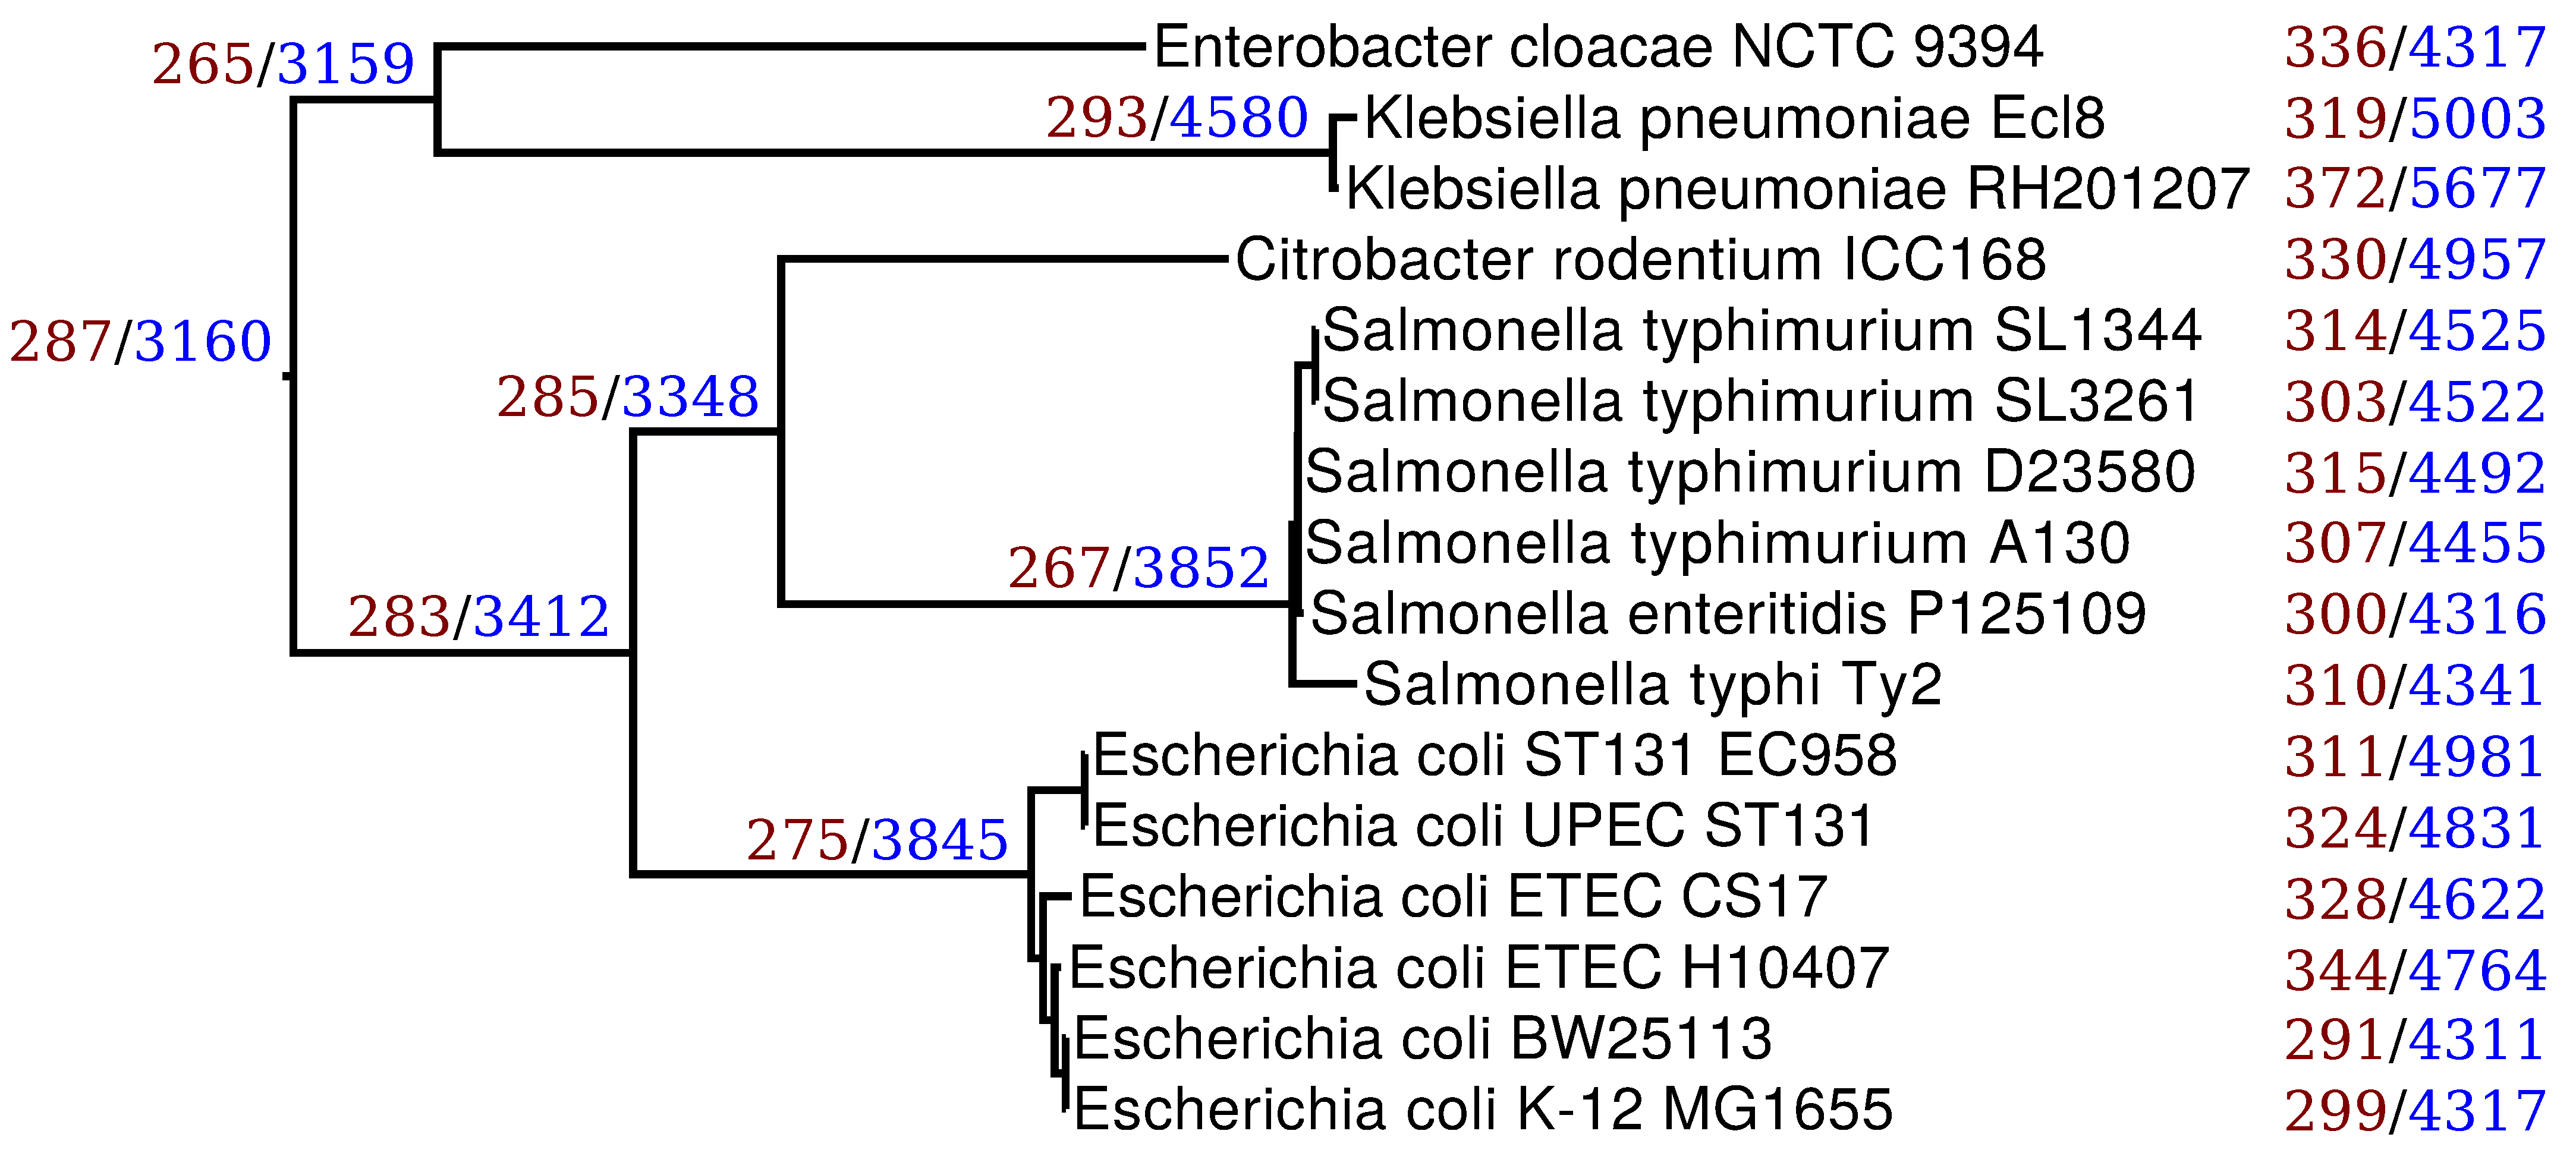
\includegraphics[scale=0.2]{phylosift-aa-raxmlbootstrap-annotated.pdf}
\caption{The tree shows the species tree in Fig.\@\ref{fig:species-tree} annotated by the number of core essential genes and core genes at each node. We used three methods to define core essential genes and core genes. The numbers at the leaves are the same using all these three methods. At the internal nodes, red shows the numbers using the intersection method, green shows the ancestral insertion index method, and turquoise shows fdollop method.}
\label{fig:annotated-speciestree}
\end{figure}

As these three methods lead to conflicting results, we compared the differences between the genes found in these three methods. For this, we compared the set of core essential genes resulted from intersection and ancestral insertion index methods. Then, we performed word enrichment analysis that was explained before on the 184 genes in intersection method and 89 genes that are core essential using ancestral insertion index and not core essential using the intersection method. Moreover, the intersection and fdollop methods and also ancestral insertion index and fdollop method were compared using the same procedure. The results are depicted in Fig.\@\ref{fig:method-difference}.

\begin{figure*}
\centering
\begin{tabular}{c c}
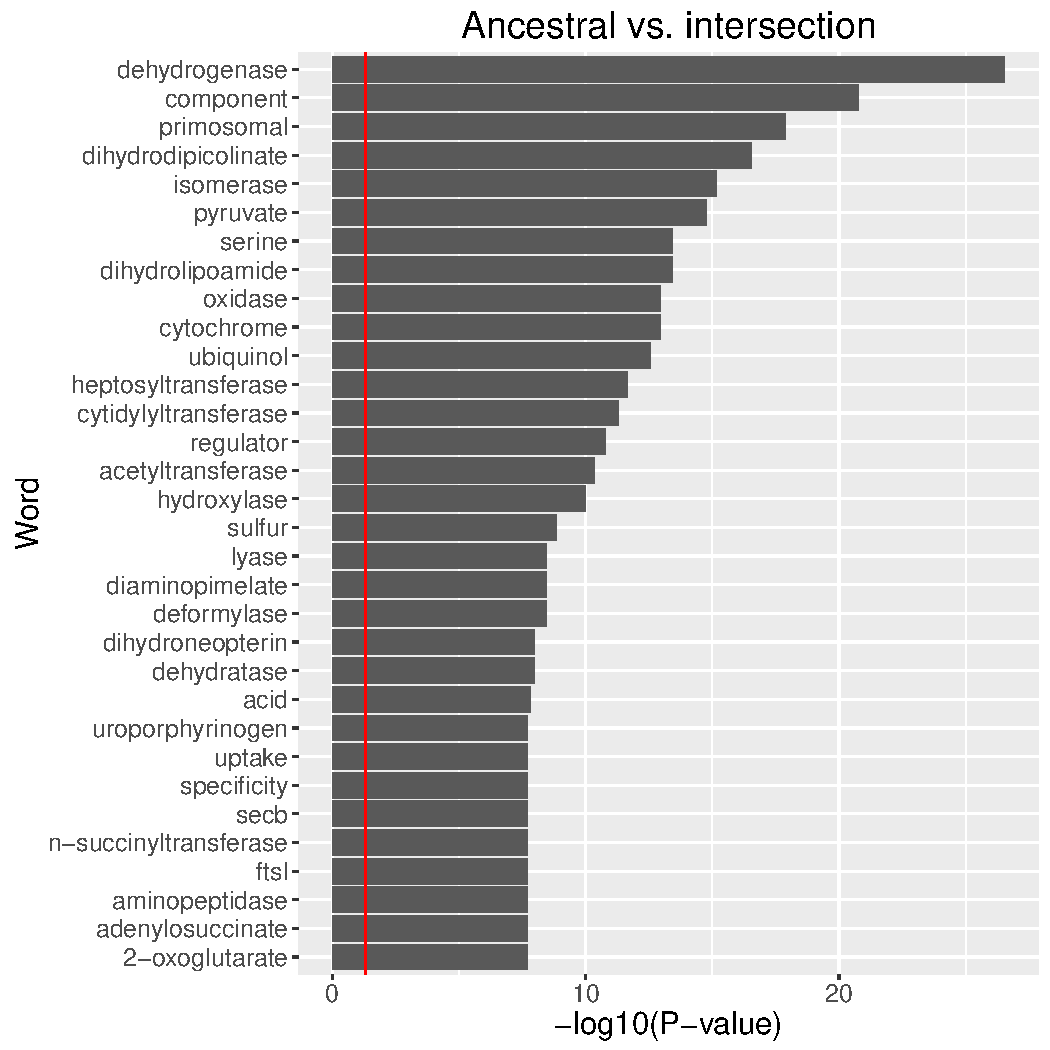
\includegraphics[scale=0.4]{ancestral-intersection-pval.pdf}&
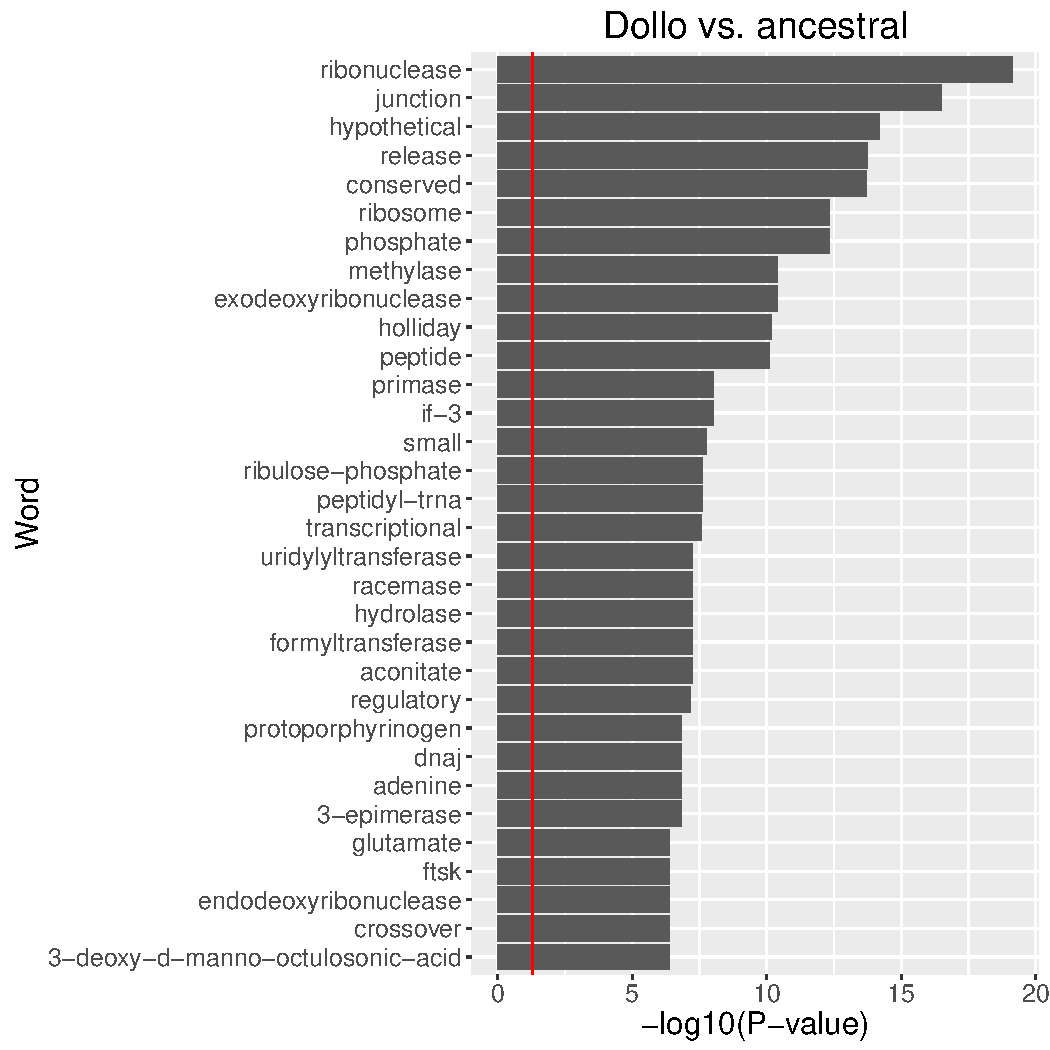
\includegraphics[scale=0.4]{dollo-ancestral-pval.pdf}\\
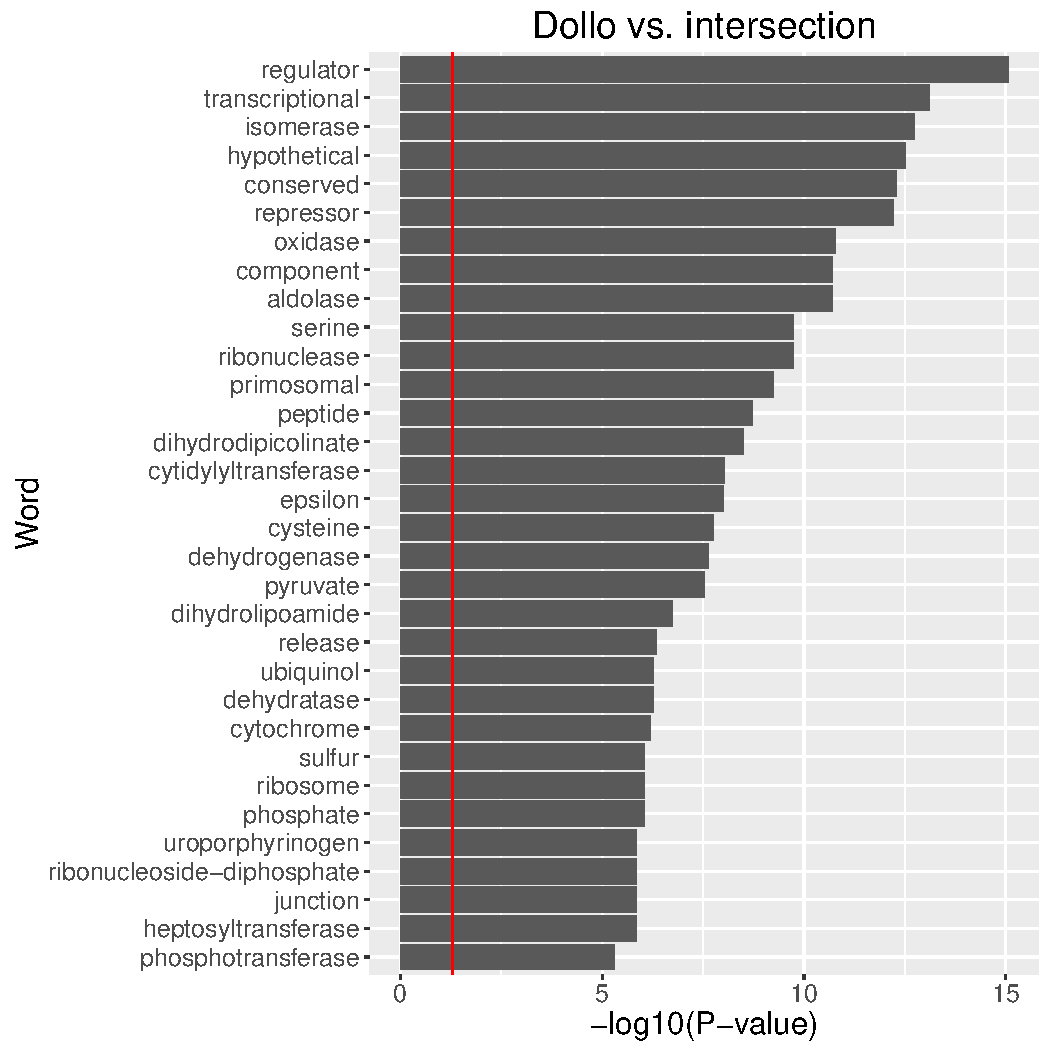
\includegraphics[scale=0.4]{dollo-intersection-pval.pdf}&
\end{tabular}
\caption{The figure shows the difference between core essential genes in intersection and ancestral insertion index methods, ancestral insertion index and fdollop methods, and intersection and fdollop methods. The red line shows P-value = 0.05. The P-values have been calculated using Fisher's exact test and then corrected using Benjamini-Hochberg-Yekutieli procedure. The top left figure shows words that are enriched in core essential genes found using ancestral insertion index method but not enriched in core essential genes found using intersection method. The top right figure shows words that are enriched in core essential genes found using fdollop method but not enriched in core essential genes found using ancestral insertion index method. The bottom left figure shows words that are enriched in core essential genes found using fdollop method but not enriched in core essential genes found using intersection method.}
\label{fig:method-difference}
\end{figure*}

\section{Materials and Methods}
\subsection{Transposon mutagenesis}\label{sec:transposoninsertion}
We studied 2 \textit{Klebsiella} strains, an \textit{Enterobacter} strain, a \textit{Citrobacter} strain, 6 \textit{Salmonella} strains, and 3 \textit{Escherichia} strains (Fig.\@ \ref{fig:species-tree}) and compared the essentiality of genes in these strains and \textit{Escherichia coli} K-12 MG1655 from another study \cite{baba_construction_2006}. These strains are all selected from Enterobacteriaceae family and a transposon mutagenesis study have been performed on them. We generated single inserted mutants using Tn5 transposon and placed the mutants in a selective media for Tn5. Then, we picked the mutants and pooled them and performed PCR enrichment using the method described in \cite{barquist_tradis_2016}. We sequenced the fragments and mapped them back to the genome to figure out the number of insertions that have been tolerated in each position of the genome. The number of insertions in a gene implies the degree of essentiality for that gene.

\subsection{Essentiality levels}\label{sec:essentiality}
The more transposon insertions we observe in a gene after sequencing the genomes, the less essential the gene is. In order to quantify the essentiality of genes, we used a measure named insertion index which is proportional to the number of insertions in a gene.

To calculate the insertion index for each gene, we summed up the number of transposon insertion sites observed in that gene. Since the lengths of the genes are different, the insertion indices were then normalised by dividing them by gene length. Our experiment is performed on different strains and the library density is different in each experiment. Therefore, in order to make the insertion indices comparable in all the strains, we normalised the insertion indices by the ratio between the number of insertions in the whole genome and the length of the genome.

Based on insertion indices, the genes were divided into four groups: essential genes, ambiguous, non-essential genes, and beneficial losses. We utilised the pipeline introduced by Barquist et al.\@ \cite{barquist_tradis_2016} to evaluate the essentiality of genes. The insertion index distribution plot has two peaks and a heavy tail as shown in Fig.\@ \ref{fig:iidist-species}. A loess curve was fitted to this distribution to find where the two peaks separate from each other. The first peak shows the genes with no or just a few insertions which are considered as essential genes. We fitted an exponential distribution to the first peak and a gamma distribution to the second one. Then, we calculated the log odds ratio for belonging to each of these distributions for each gene. The region that has log odds value between -2 and 2 is called the ambiguous region, the genes belonging to the first peak are essential and the rest of the genes are not essential. Among genes that are not essential, any gene for which the value of the cumulative distribution function for the gamma distribution is greater than or equal to 0.99 is considered as a beneficial loss and the other genes are non-essential genes.

\begin{figure*}
\centering
\begin{tabular}{c c c}
\includegraphics[page=1, scale=0.25]{essentiality.pdf}&
\includegraphics[page=2, scale=0.25]{essentiality.pdf}&
\includegraphics[page=3, scale=0.25]{essentiality.pdf}\\
\includegraphics[page=4, scale=0.25]{essentiality.pdf}&
\includegraphics[page=5, scale=0.25]{essentiality.pdf}&
\includegraphics[page=6, scale=0.25]{essentiality.pdf}\\
\includegraphics[page=7, scale=0.25]{essentiality.pdf}&
\includegraphics[page=8, scale=0.25]{essentiality.pdf}&
\includegraphics[page=9, scale=0.25]{essentiality.pdf}\\
\includegraphics[page=10, scale=0.25]{essentiality.pdf}&
\includegraphics[page=11, scale=0.25]{essentiality.pdf}&
\includegraphics[page=12, scale=0.25]{essentiality.pdf}\\
&\includegraphics[page=13, scale=0.25]{essentiality.pdf}&\\
\end{tabular}
\caption{Plots show the insertion index distribution for each genome. The plots are divided into 4 regions using red lines. These regions from left to right are: essential, ambiguous, non-essential, and beneficial loss.}
\label{fig:iidist-species}
\end{figure*}

\subsection{Bias correction}\label{sec:biascorrection}
We observed a distance from origin of replication bias and also a positional bias within genes. Hence, these biases needed to be corrected before inferring the essentiality of genes from their insertion indices. We did not include genes shorter than 100 base-pairs in our study as they might not be targeted by any transposon due to their shortness. 

To overcome the distance from origin of replication bias, we divided the value of insertion index for a gene in a specific position by the predicted value by loess for that position. This value was then multiplied by the average insertion index. To overcome the positional bias within genes, we calculated the insertion index for genes by ignoring $5\%$ from the 5' end and $20\%$ from the 3' end of the genes. The insertion index distribution for each genome after correcting for distance from the origin of replication bias and bias towards the position of insertion within genes is depicted in Fig.\@ \ref{fig:iidist-species-normalised}.

\begin{figure*}
\centering
\begin{tabular}{c c c}
\includegraphics[page=1, scale=0.25]{essentiality-normalised.pdf}&
\includegraphics[page=2, scale=0.25]{essentiality-normalised.pdf}&
\includegraphics[page=3, scale=0.25]{essentiality-normalised.pdf}\\
\includegraphics[page=4, scale=0.25]{essentiality-normalised.pdf}&
\includegraphics[page=5, scale=0.25]{essentiality-normalised.pdf}&
\includegraphics[page=6, scale=0.25]{essentiality-normalised.pdf}\\
\includegraphics[page=7, scale=0.25]{essentiality-normalised.pdf}&
\includegraphics[page=8, scale=0.25]{essentiality-normalised.pdf}&
\includegraphics[page=9, scale=0.25]{essentiality-normalised.pdf}\\
\includegraphics[page=10, scale=0.25]{essentiality-normalised.pdf}&
\includegraphics[page=11, scale=0.25]{essentiality-normalised.pdf}&
\includegraphics[page=12, scale=0.25]{essentiality-normalised.pdf}\\
&\includegraphics[page=13, scale=0.25]{essentiality-normalised.pdf}&\\
\end{tabular}
\caption{Plots show the insertion index distribution for each genome after correcting for distance from the origin of replication bias and bias towards the position of insertion within genes. The plots are divided into 4 regions using red lines. These regions from left to right are: essential, ambiguous, non-essential, and beneficial loss.}
\label{fig:iidist-species-normalised}
\end{figure*}

\subsection{Conservation classes}\label{sec:conservationclasses}
To study whether each gene in the 13 organisms is conserved we proposed a program that clusters homologous proteins. This program uses Jackhmmer from HMMER package~\cite{eddy_accelerated_2011} to compare protein sequences. It first compares a set of query proteins against all given proteins and clusters homologous proteins using Jackhmmer. Then, it selects all sequences that were not selected in the first step and compares them together and clusters those protein sequences. In the next step, it breaks down large clusters by using Jackhmmer with more stringent parameters within the clusters and also merges clusters which have a single member by running Jackhmmer with more permissive parameters. Finally, the program merges overlapping sequences in each cluster and combines similar clusters. The program is summarised in Fig.\@ \ref{fig:homclust} and the distribution of cluster lengths after clustering the genes of 13 strains under study is plotted in Fig.\@ \ref{fig:homclust-results}.

\begin{figure}
\includegraphics[scale=0.2]{homclust.pdf}
\caption{The steps of our proposed algorithm for clustering homologous genes.}
\label{fig:homclust}
\end{figure}

We divided the clusters of homologous genes into three groups based on their conservation. Genus specific clusters contain genes that are present only in one genus, the genes in single copy clusters are present in more than one genus and more than 70\% of them are not duplicated, and  the genes in multi-copy clusters are present in more than one genus and less than 70\% of them are not duplicated. These three groups are depicted in Fig.\@ \ref{fig:homclust-results}.

\begin{figure}
\includegraphics[scale=0.3]{cluster-size-dist.pdf}
\caption{Size distribution for all clusters of homologous genes. Genus specific genes are genes that are present only in one genus, single copy genes are present in more than one genus and more than 70\% of them are not duplicated, and multi-copy genes are present in more than one genus and less than 70\% of them are not duplicated.}
\label{fig:homclust-results}
\end{figure}

\subsection{Defining core and core essential genes}\label{sec:core}
We used three different methods for defining core and core essential genes: intersection, ancestral insertion index, and Dollo law. These three methods are explained in what follows.

The first method was intersecting over core genes and core essential genes, so, genes are core in a node if and only if they are core in all the descendants of that node and are core essential if and only if they are core essential in all the descendants of that node.

The second method which is called ancestral insertion index uses intersection for core genes but a different definition for core essential genes. In this method, we averaged over the insertion indices of the pair of closest children of the ancestral node. We repeated this and averaged the averages until we reached the ancestral node. Then, we plotted the insertion indices and fitted an exponential and a gamma distribution to the plot as described in Section~\ref{sec:essentiality} and found the essential genes at that level.

The third method is using Dollo law to define core genes and core essential genes. This method, assumes that the gain of genes (gain of essentiality) is highly improbable, so it tries to have up to one occurrence of gain of genes (gain of essentiality) and minimise the number of times that a gene (the essentiality of a gene) has been lost. Using this method, we can predict which genes were present in the common ancestor of our strains and which genes were essential in it.

\section*{Acknowledgments}
%
%
%\nolinenumbers

%This is where your bibliography is generated. Make sure that your .bib file is actually called library.bib
\bibliography{references}

%This defines the bibliographies style. Search online for a list of available styles.
\bibliographystyle{abbrv}

\end{document}

